%\documentclass[a4paper]{article}
% #### CONFIGURACIONES ####
\documentclass[12pt,a4paper,oneside]{book} % tamaño 12
%\usepackage[spanish]{babel}
\usepackage[spanish, es-tabla]{babel}
\usepackage[utf8x]{inputenc}
\usepackage[usenames]{color}
\usepackage[table,xcdraw]{xcolor}
\usepackage{tikz} % grafos
\usetikzlibrary{arrows,shapes,positioning,shadows,trees}
\usepackage{amsmath} % códigos
\usepackage{setspace} %interlineado algoritmo
\usepackage{algorithm}
%\usepackage{algorithmicx}
\usepackage{algpseudocode}
\usepackage{rotating} % rotate graphics
\usepackage{pdflscape} % automatic rotation of the page 
\usepackage{longtable}
\algdef{SE}[DOWHILE]{Do}{doWhile}{\algorithmicdo}[1]{\algorithmicwhile\ #1}%
\usepackage[hidelinks]{hyperref}
\usepackage{subfig} % Para poner imágenes
\usepackage{graphicx} % para poner dos imágenes juntas
\usepackage[colorinlistoftodos]{todonotes}
\usepackage{anysize}
\marginsize{4cm}{2.5cm}{2.5cm}{2.5cm}
% Márgenes {izquierda}{derecha}{arriba}{abajo}.
\usepackage{mathptmx}% http://ctan.org/pkg/mathptmx Times new roman
\usepackage{amsfonts}% Para expresiones matemáticas
%\usepackage{setspace} % interlineado
\renewcommand{\baselinestretch}{1.5} % Interlineado
\usepackage{enumerate}% para los enumerate
\usepackage{fancyhdr}
\pagestyle{fancy}
\usepackage[none]{hyphenat} %saltos y justificación texto
\usepackage{float}
\usepackage{tikz}
\usetikzlibrary{calc}
\usepackage{changepage}
\usepackage{ragged2e}
\usepackage{tabularx} % Para meter tablas que no excedan los márgenes del papel
\usepackage{fancyhdr}

%%%%%%%%%%%%%%%%%%%%%%%
%%%%%%%% XML %%%%%%%%%%
\usepackage{listings}

\usepackage{appendix}
% cambiar apéndices por anexos
\renewcommand{\appendixname}{Anexos}
\renewcommand{\appendixtocname}{Anexos}
\renewcommand{\appendixpagename}{Anexos}
%\newcommand{\specialcell}[1]{\begin{tabular}{@{}c@{}}#1\end{tabular}}
 \everycr={\noalign{\global\advance\stepno by 1}}%
 
\usepackage{color}
\definecolor{gray}{rgb}{0.4,0.4,0.4}
\definecolor{darkblue}{rgb}{0.0,0.0,0.6}
\definecolor{cyan}{rgb}{0.0,0.6,0.6}

\usepackage[export]{adjustbox} % -- imagenes y cosas
\usepackage{enumitem}
\newlist{tabitemize}{itemize}{1}
\setlist[tabitemize]{label=\textbullet,nosep,after=\strut,align=parleft,leftmargin=*,}

\lstset{
  basicstyle=\ttfamily,
  columns=fullflexible,
  showstringspaces=false,
  commentstyle=\color{gray}\upshape
}

\lstdefinelanguage{XML}
{
  morestring=[b]",
  morestring=[s]{>}{<},
  morecomment=[s]{<?}{?>},
  stringstyle=\color{black},
  identifierstyle=\color{darkblue},
  keywordstyle=\color{cyan},
  morekeywords={id,tx,ty,tz,rx,ry,rz,scale,file,type}% list your attributes here
}
%%%%%%%%%%%%%%%%%%%%%%%%%%%%
%%%%%%%%%%%%% COLOR %%%%%%%%
\definecolor{palegreen}{rgb}{0.6, 0.98, 0.6}
\definecolor{palegoldenrod}{rgb}{0.93, 0.91, 0.67}

\makeatletter
\def\BState{\State\hskip-\ALG@thistlm}
\makeatother

%%%% Carpeta de las figuras


% Logo de la uex en el header de todas las páginas
%\rhead{\begin{picture}(0,0) \put(0,0){
\includegraphics[width=1cm,natwidth=124,natheight=163]{pictures/logouex_transp.png}}
%\end{picture}}
\fancypagestyle{plain}{
	\fancyhf{}
	\rhead{
\includegraphics[width=1cm,natwidth=124,natheight=163]{pictures/logouex_transp.png}}
	\fancyhead[L]{\leftmark}
	\headsep = -1cm
}
\pagestyle{fancy}
\fancyhf{}
\rhead{
\includegraphics[width=1cm,natwidth=124,natheight=163]{pictures/logouex_transp.png}}
\fancyhead[L]{\leftmark}
\headsep = 2cm
	
\begin{document}
\sloppy
\pagebreak
%http://tex.stackexchange.com/questions/129º088/create-a-frame-for-a-title-page
% ### DALE CAÑA PRIMO ###
\makeatletter
\begin{titlepage}
	\begin{adjustwidth}{-1.5cm}{0cm}
		\begin{tikzpicture}[remember picture, overlay]
		\usetikzlibrary{calc}
		\draw[line width = 1.5pt] ($(current page.north west) + (1in,-1in)$) rectangle ($(current page.south east) + (-1in,1in)$);
		\end{tikzpicture}

		\vspace{-3em}
		\hspace{-0.5em}
		\begin{minipage}{0.45\textwidth}
			\begin{flushleft}
				
\includegraphics[width=1.75cm,natwidth=124,natheight=163]{pictures/logouex_transp.png}
			\end{flushleft}
		\end{minipage}

		\vspace{-5.5em}
		\hspace{20em}
		\begin{minipage}{0.45\textwidth}
			\begin{flushright} % width=0.8\textwidth,height=0.8\textheight,keepaspectratio
				
\includegraphics[width=4cm, natwidth=233,natheight=135]{pictures/logoEpcc.png}
			\end{flushright}
		\end{minipage}\\[1.5cm]

		\begin{center}
			% Upper part of the page
			\textsc{\LARGE UNIVERSIDAD DE EXTREMADURA}\\[4cm]

			\textsc{\Large Escuela Politécnica}\\[0.5cm]
			\textsc{\Large Grado en Ingeniería Informática en Ingeniería de Software}\\[3cm]
			\textsc{\Large Trabajo Fin de Grado}\\[0.5cm]
%			{ \large \bfseries }\\[4.0cm]
			\vfill
			% Bottom of the page
			{\large}
		\end{center}
	\end{adjustwidth}
\end{titlepage}
\thispagestyle{empty}
\begin{titlepage}
	\begin{adjustwidth}{-1.5cm}{0cm}
		\begin{tikzpicture}[remember picture, overlay]
		\usetikzlibrary{calc}
		\draw[line width = 1.5pt] ($(current page.north west) + (1in,-1in)$) rectangle ($(current page.south east) + (-1in,1in)$);
		\end{tikzpicture}

		\vspace{-3em}
		\hspace{-0.5em}
		\begin{minipage}{0.55\textwidth}
			\begin{flushleft}F1
				
\includegraphics[width=1.75cm,natwidth=124,natheight=163]{pictures/logouex_transp.png}
			\end{flushleft}
		\end{minipage}

		\vspace{-5.5em}
		\hspace{20em}
		\begin{minipage}{0.45\textwidth}
			\begin{flushright}
				
\includegraphics[width=4cm,natwidth=233,natheight=135]{pictures/logoEpcc.png}
			\end{flushright}
		\end{minipage}\\[1.5cm]

		\begin{center}


			% Upper part of the page
			\textsc{\LARGE UNIVERSIDAD DE EXTREMADURA}\\[3cm]

			\textsc{\Large Escuela Politécnica}\\[0.5cm]
			\textsc{\Large Grado en Ingeniería Informática en Ingeniería de Software}\\[2.5cm]
			\textsc{\Large Trabajo Fin de Grado}\\[0.5cm]
			{ \large \bfseries Extracción del contexto de ejecución del usuario}\\[4.0cm]
			{ \large \bfseries Autor: Alberto de la Fuente Cruz}\\[0.5cm]
			{ \large \bfseries Tutor: Juan Manuel Murillo}\\[0.5cm]
			\vfill
			% Bottom of the page
			{\large}
		\end{center}
	\end{adjustwidth}
\end{titlepage}
%\makeatother
\thispagestyle{empty}
%\newpage
%\thispagestyle{empty}
% #### DOCUMENTO ####
\chapter*{Resumen}
\thispagestyle{empty}
Lorem ipsum dolor sit amet, consectetur adipiscing elit, sed do eiusmod tempor incididunt ut labore et dolore magna aliqua. Ut enim ad minim veniam, quis nostrud exercitation ullamco laboris nisi ut aliquip ex ea commodo consequat. Duis aute irure dolor in reprehenderit in voluptate velit esse cillum dolore eu fugiat nulla pariatur. Excepteur sint occaecat cupidatat non proident, sunt in culpa qui officia deserunt mollit anim id est laborum.

Sed ut perspiciatis unde omnis iste natus error sit voluptatem accusantium doloremque laudantium, totam rem aperiam, eaque ipsa quae ab illo inventore veritatis et quasi architecto beatae vitae dicta sunt explicabo. Nemo enim ipsam voluptatem quia voluptas sit aspernatur aut odit aut fugit, sed quia consequuntur magni dolores eos qui ratione voluptatem sequi nesciunt. Neque porro quisquam est, qui dolorem ipsum quia dolor sit amet, consectetur, adipisci velit, sed quia non numquam eius modi tempora incidunt ut labore et dolore magnam aliquam quaerat voluptatem. Ut enim ad minima veniam, quis nostrum exercitationem ullam corporis suscipit laboriosam, nisi ut aliquid ex ea commodi consequatur? Quis autem vel eum iure reprehenderit qui in ea voluptate velit esse quam nihil molestiae consequatur, vel illum qui dolorem eum fugiat quo voluptas nulla pariatur?
\thispagestyle{empty}
%\chapter*{Abstract}
%\thispagestyle{empty}
%EL RESUMEN EN INGLÉS
\pagenumbering{roman}
\setcounter{page}{1}
\tableofcontents
%\pagebreak
%\newpage
\listoftables
%\newpage
\listoffigures
%\newpage


%%%%%%% ESTRUCTURA DEL TFG %%%%%%%%%%%%%%
% A.PORTADA (según la estructura indicada a continuación)
% B.CONTRAPORTADA (según la estructura indicada a continuación)
% C.ÍNDICE GENERAL DE CONTENIDOS
% D.ÍNDICE DE TABLAS
% E.ÍNDICE DE FIGURAS
% F.RESUMEN (Podrá incluirse también en inglés, si así lo indica el Tutor1)
% G.CUERPO DEL TRABAJO (según la estr
% uctura indicada a continuación)
% H.REFERENCIAS BIBLIOGRÁFICAS
% (Según norma ISO690)
% I.ANEXOS, si los hubiera
%%%%%%%%%%%%%%%%%%%%%%%%%%%%%%%%%%%%%%%
%%%%%% Cuerpo del trabajo
% 1.INTRODUCCIÓN
% 2.OBJETIVOS
% 3.ANTECEDENTES / ESTADO DEL ARTE
% 4.MÉTODOLOGÍA
% 5.IMPLEMENTACIÓN Y DESARROLLO (Cuando proceda)
% 6.RESULTADOS Y DISCUSIÓN
% 7.CONCLUSIONES
%%%%%%%%%%%%%%%%%%%%%%%%%%%%%%%%%%%%%%%%%%%
%%%%%%%%%%%%%%%%%%%%%%%%%%%%%%%%%%%%%%%%%%%
% Tamaño: Normalizado UNE A-4, salvo planos.
% Tipo y tamaño de letra del texto: Times New Roman 12 pt, Arial 12 pt o similar.
% Interlineado del texto: 1,5 líneas.
% Márgenes del texto: Superior, Inferior y Derecha, 2,5 cm; Izquierda, 4 cm.
% Numeración de páginas en margen inferior derecha y tamaño 8 pt.
% Las  figuras  serán  numeradas  y  tituladas  debajo  de  las  mismas  (indicando  su  fuente  si  no  son  de  elaboración
% propia).
% Las  tablas  serán  numeradas  y  tituladas  encima  de  las  mismas  (indicando  su  fuente  si  no  son  de  elaboración
% propia).
%%%%%%%%%%%%%%%%%%%%%%%%%%%%%%%%%%%%%%%%%%%
%%%%%%%%%%%%%%%%%%%%%%%%%%%%%%%%%%%%%%%%%%%
%%%%%%%%%%%%%%%%%%%%%%%%%%%%%%%%%%%%%%%%%%%
%%%%%%%%%%%%%%%%%%%%%%%%%%%%%%%%%%%%%%%%%%%


\pagenumbering{arabic}
\pagestyle{fancy}
\setcounter{page}{1}

\chapter{Introducción}
El ejercicio propuesto se plantea del siguiente modo. Es objetivo del proyecto ser capaces de desarrollar una aplicación android capaz de escuchar lo que el usuario \textit{dice} al teléfono, con esto nos referimos a toda la información que surge del usuario al interactuar con su dispositivo y que por el momento pasa desapercibida. Esta información, sea del tipo que sea nos aportan un grado más de información acerca de nuestros usuarios, siendo el fin último ser capaces de registrar sus rutinas de comportamiento, uso y costumbres interactuando con la tecnología con el fin de inferir patrones sobre el usuario. 

Es tarea del proyecto la parte relacionada con la recogida de información del sistema, actividad que nos ocupará en su estudio y desarrollo todo el recorrido del trabajo. 
\chapter{Estado del Arte}
-- aquí hablaremos sobre las distintas aproximaciones al problema en términos de implementación. 

\chapter{Requisitos del proyecto}
En esta capítulo se analiza el problema planteado por el proyecto y se detalla su descomposición como requisitos de un sistema software. No hay que perder de vista que nuestro objetivo final será monitorizar las aplicaciones del usuario y registrar información acerca de cómo éste interactúa con el medio.
\newpage
\section{Requisitos}
\subsection{Requisitos funcionales}
El sistema deberá: 
\begin{itemize}
  \item Registrar cada aplicación que lanza el usuario, con información suficiente que permita identificarla. 
  \item Aportar un contexto temporal de cuando las aplicaciones son ejecutadas, esto es, fecha y hora exactas. 
  \item Incluyendo lo anterior, registrar el uso dado a aplicaciones relacionadas con, comunicación, mensajería instantánea, búsqueda web,redes sociales y por último sensores. 
  \item Dentro de comunicación se incluye la aplicación de Gmail, Mensajes (sms) y el Teléfono. 
  \item Dentro mensajería instantánea prestaremos atención a Telegram, Whatsapp Messenger y Facebook Messenger. 
  \item Como aplicaciones relacionadas con la búsqueda en la web estarán la Chrome Browser y Google Search. 
  \item En las aplicaciones de redes sociales; Twitter, Facebook e Instagram.
  \item Los sensores que escucharemos serán el emisor de GPS, acelerómetro, presión, giroscopio y temperatura.
\subsubsection{Aplicaciones de comunicación}
  \item En  \textbf{Gmail} capturar, la dirección de correo del emisor. 
  \item La dirección de correo del receptor(es). 
  \item El asunto del correo electrónico. 
  \item El contenido, cuerpo de dicho correo. 
  \item En \textbf{Mensajes} se deberá capturar, el destinatario. 
  \item El cuerpo del mensaje. 
  \item En \textbf{Teléfono} se deberá capturar, el destinatario de la llamada. 
  \item Tiempo total invertido en ella. 
\subsubsection{Aplicaciones de mensajería instantánea}
  \item En \textbf{Telegram} capturar, el nombre del contacto o grupo interlocutor. 
  \item Los mensajes enviados en la conversación por parte del usuario. 
  \item En \textbf{Whatsapp} capturar, el nombre del contacto o grupo interlocutor. 
  \item Los mensajes enviados en la conversación por parte del usuario. 
  \item En \textbf{Facebook Messenger} capturar, el nombre del contacto o grupo interlocutor. 
  \item Los mensajes enviados en la conversación por parte del usuario. 
\subsubsection{Aplicaciones de búsqueda en la web}
  \item En \textbf{Chrome} capturar el objeto de búsqueda. 
  \item El tiempo invertido en la aplicación. 
  \item En \textbf{Búsqueda de google} el objeto de búsqueda. 
\subsubsection{Aplicaciones de redes sociales}
  \item En \textbf{Twitter} capturar, el nombre de los perfiles visitados. 
  \item Los los \textit{retuits} realizados. 
  \item Los \textit{me gusta} dados. 
  \item El contenido de los mensajes directos. 
  \item Interlocutor de esos mensajes directos. 
  \item En \textbf{Facebook} capturar, el nombre de los perfiles visitados. 
  \item Los comentarios hechos en dichos perfiles. 
  \item Los estados compartidos dentro de la red social. 
  \item Las subidas de fotos y su título. 
  \item Los \textit{me gusta} dados. 
  \item En \textbf{Instagram} capturar, el nombre de los perfiles visitados. 
  \item Los comentarios hechos en dichos perfiles. 
  \item Las subidas de fotos y su descripción. 
  \item Los \textit{me gusta} dados.
  \item Los mensajes directos. 
  \item El interlocutor de esos mensajes directos. 
\end{itemize}
\subsubsection{Sensores}
\begin{itemize}
  \item Del sensor relacionado con la ubicación \textbf{GPS} deberemos registrar cada cambio de coordenadas que registre el teléfono. 
  \item Mediante el \textbf{acelerómetro} registraremos los cambios en la aceleración del teléfono. 
  \item Con el sensor de \textbf{presión} registraremos los cambios de altitud del teléfono. 
  \item Con el \textbf{giroscopio} para detectar y registrar  los movimientos que realiza el teléfonpo. 
  \item El sensor de \textbf{temperatura} nos permitirá registrar, como no, la temperatura ambiente del dispositivo. 
\end{itemize}
\newpage
\subsection{Requisitos no funcionales}
\begin{itemize}
	\item Versión. El sistema deberá soportar una versión limpia de Android 8.0. 
	\item Eficiencia. Dado que el sistema debe registrar en tiempo real toda la información generada por el usuario, deberá ser capaz de capturarla en tiempo real, al mismo tiempo que se analiza y almacena. 
	\item Privacidad. El usuario deberá autorizar explícitamente al software desarrollado permisos de accesibilidad, de modo que sea consciente de que existe una aplicación monitorizando parte de su actividad.
	\item Robustez. Debido a que el sistema debe estar constantemente capturando, el software debe ser tolerante a fallos y mantener el servicio siempre disponible.  
	\item Seguridad. La base de datos local deberá estar protegida ante el acceso indebido a los datos. 
\end{itemize}
\break
\chapter{Análisis}
Para centrar el problema y enfocar los requisitos a un proceso que nos lleve a obtener un proyecto de ingeniería, haremos uso de distintos diagramas que nos ayudaran a resolver el problema y plantear una solución. Así en el capítulo nos encontramos con los diagramas de casos de uso, indicando las tareas que debe resolver el sistema, y un diagrama de arquitectura a alto nivel que plantea una solución inicial. 
\pagebreak
\section{Diagramas de Casos de Uso}
Si nos fijamos en como está planteado el proyecto, no tendremos un usuario como tal, si no que nos aprovecharemos de los movimientos de este para registrar de forma pasiva lo que hace. 
\newline
\newline
Plantearemos entonces los casos de uso desde dos puntos de vista, el primero será aquel en el que usuario será el actor interaccionando con el teléfono y se dispara la recogida de información. 
\newline 
\newline
El segundo punto de vista en el que nos basaremos será aquel donde el actor será la propia recogida de información, empleando para ello sucesivos casos de uso que conformarán la lógica de negocio general del sistema. 
\newline 
\newline 
Aquí tenemos los casos de uso del usuario entonces; 
%%% ------ 
\begin{figure}[H]
	\begin{center}
		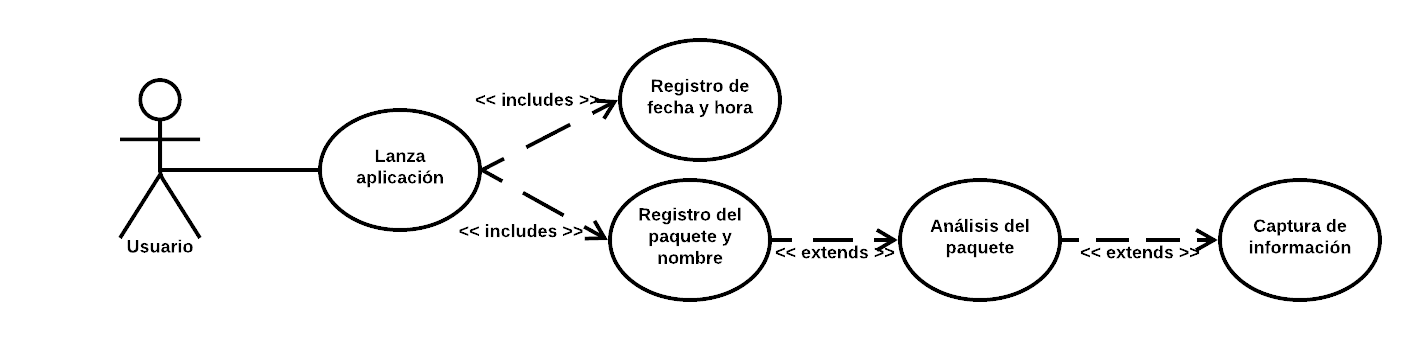
\includegraphics[scale=0.30]{pictures/usecases/usecases01.png} % include ./img/imagen.[pdf|png|jgp] si es pdflatex o ./img/imagen.eps si es latex
	\end{center}
	\caption[Casos de uso 01]{Casos de uso próximos al usuario.}
\end{figure}
%%% ------
\pagebreak
Siendo los casos de uso desde el punto de vista de la captura de información los siguientes. Si nos centramos en el apartado de aplicaciones de comunicación; 
%%% ------ 
\begin{figure}[H]
	\begin{center}
		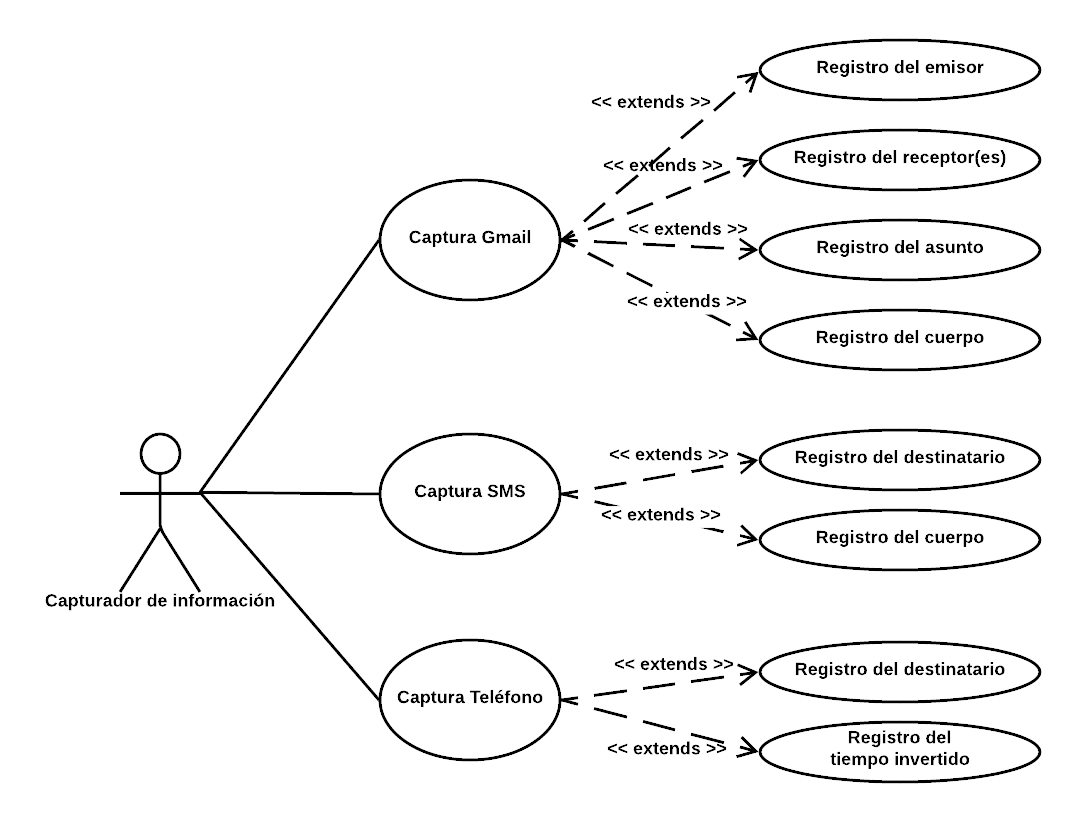
\includegraphics[scale=0.30]{pictures/usecases/usecases02.png} % include ./img/imagen.[pdf|png|jgp] si es pdflatex o ./img/imagen.eps si es latex
	\end{center}
	\caption[Casos de uso 02]{CU Apps de comunicación.}
\end{figure}
%%% ------
En el grupo de mensajería instantánea.
%%% ------ 
\begin{figure}[H]
	\begin{center}
		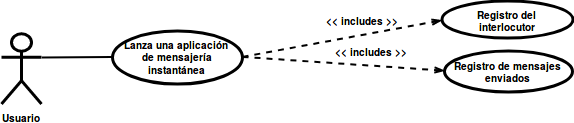
\includegraphics[scale=0.30]{pictures/usecases/usecases03.png} % include ./img/imagen.[pdf|png|jgp] si es pdflatex o ./img/imagen.eps si es latex
	\end{center}
	\caption[Casos de uso 03]{CU Apps de mensajería.}
\end{figure}
%%% ------
Aplicaciones de navegación y consulta de la web. 
%%% ------ 
\begin{figure}[H]
	\begin{center}
		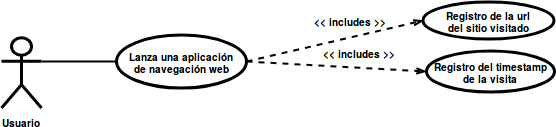
\includegraphics[scale=0.30]{pictures/usecases/usecases04.png} % include ./img/imagen.[pdf|png|jgp] si es pdflatex o ./img/imagen.eps si es latex
	\end{center}
	\caption[Casos de uso 04]{CU Apps de navegación web.}
\end{figure}
%%% ------
Si nos fijamos ahora en las aplicaciones de redes sociales, tenemos los siguientes casos de uso; 
%%% ------ 
\begin{figure}[H]
	\begin{center}
		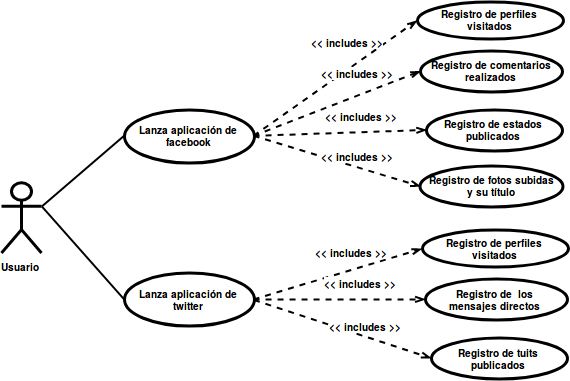
\includegraphics[scale=0.30]{pictures/usecases/usecases05.png} % include ./img/imagen.[pdf|png|jgp] si es pdflatex o ./img/imagen.eps si es latex
	\end{center}
	\caption[Casos de uso 05]{CU Apps RRSS.}
\end{figure}
%%% ------
Por último, en el apartado de los sensores, donde el actor será el capturador de la información de los sensores; 
%%% ------ 
\begin{figure}[H]
	\begin{center}
		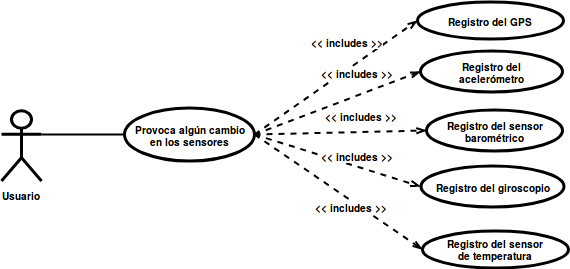
\includegraphics[scale=0.30]{pictures/usecases/usecases06.png} % include ./img/imagen.[pdf|png|jgp] si es pdflatex o ./img/imagen.eps si es latex
	\end{center}
	\caption[Casos de uso 06]{CU Sensores.}
\end{figure}
%%% ------
\pagebreak
\section{Arquitectura de alto nivel}
Teniendo claro cual es el propósito de nuestro sistema, debemos plantearnos cuales serán los elementos que, interactuando entre ellos, resuelvan el problema final. 
\newline 
\newline
 
%----------- P A N O R A M I C O -------------------------------------------------
 \begin{landscape}
\begin{figure}[ht]
  \begin{center} \setlength{\unitlength}{0.0105in}
     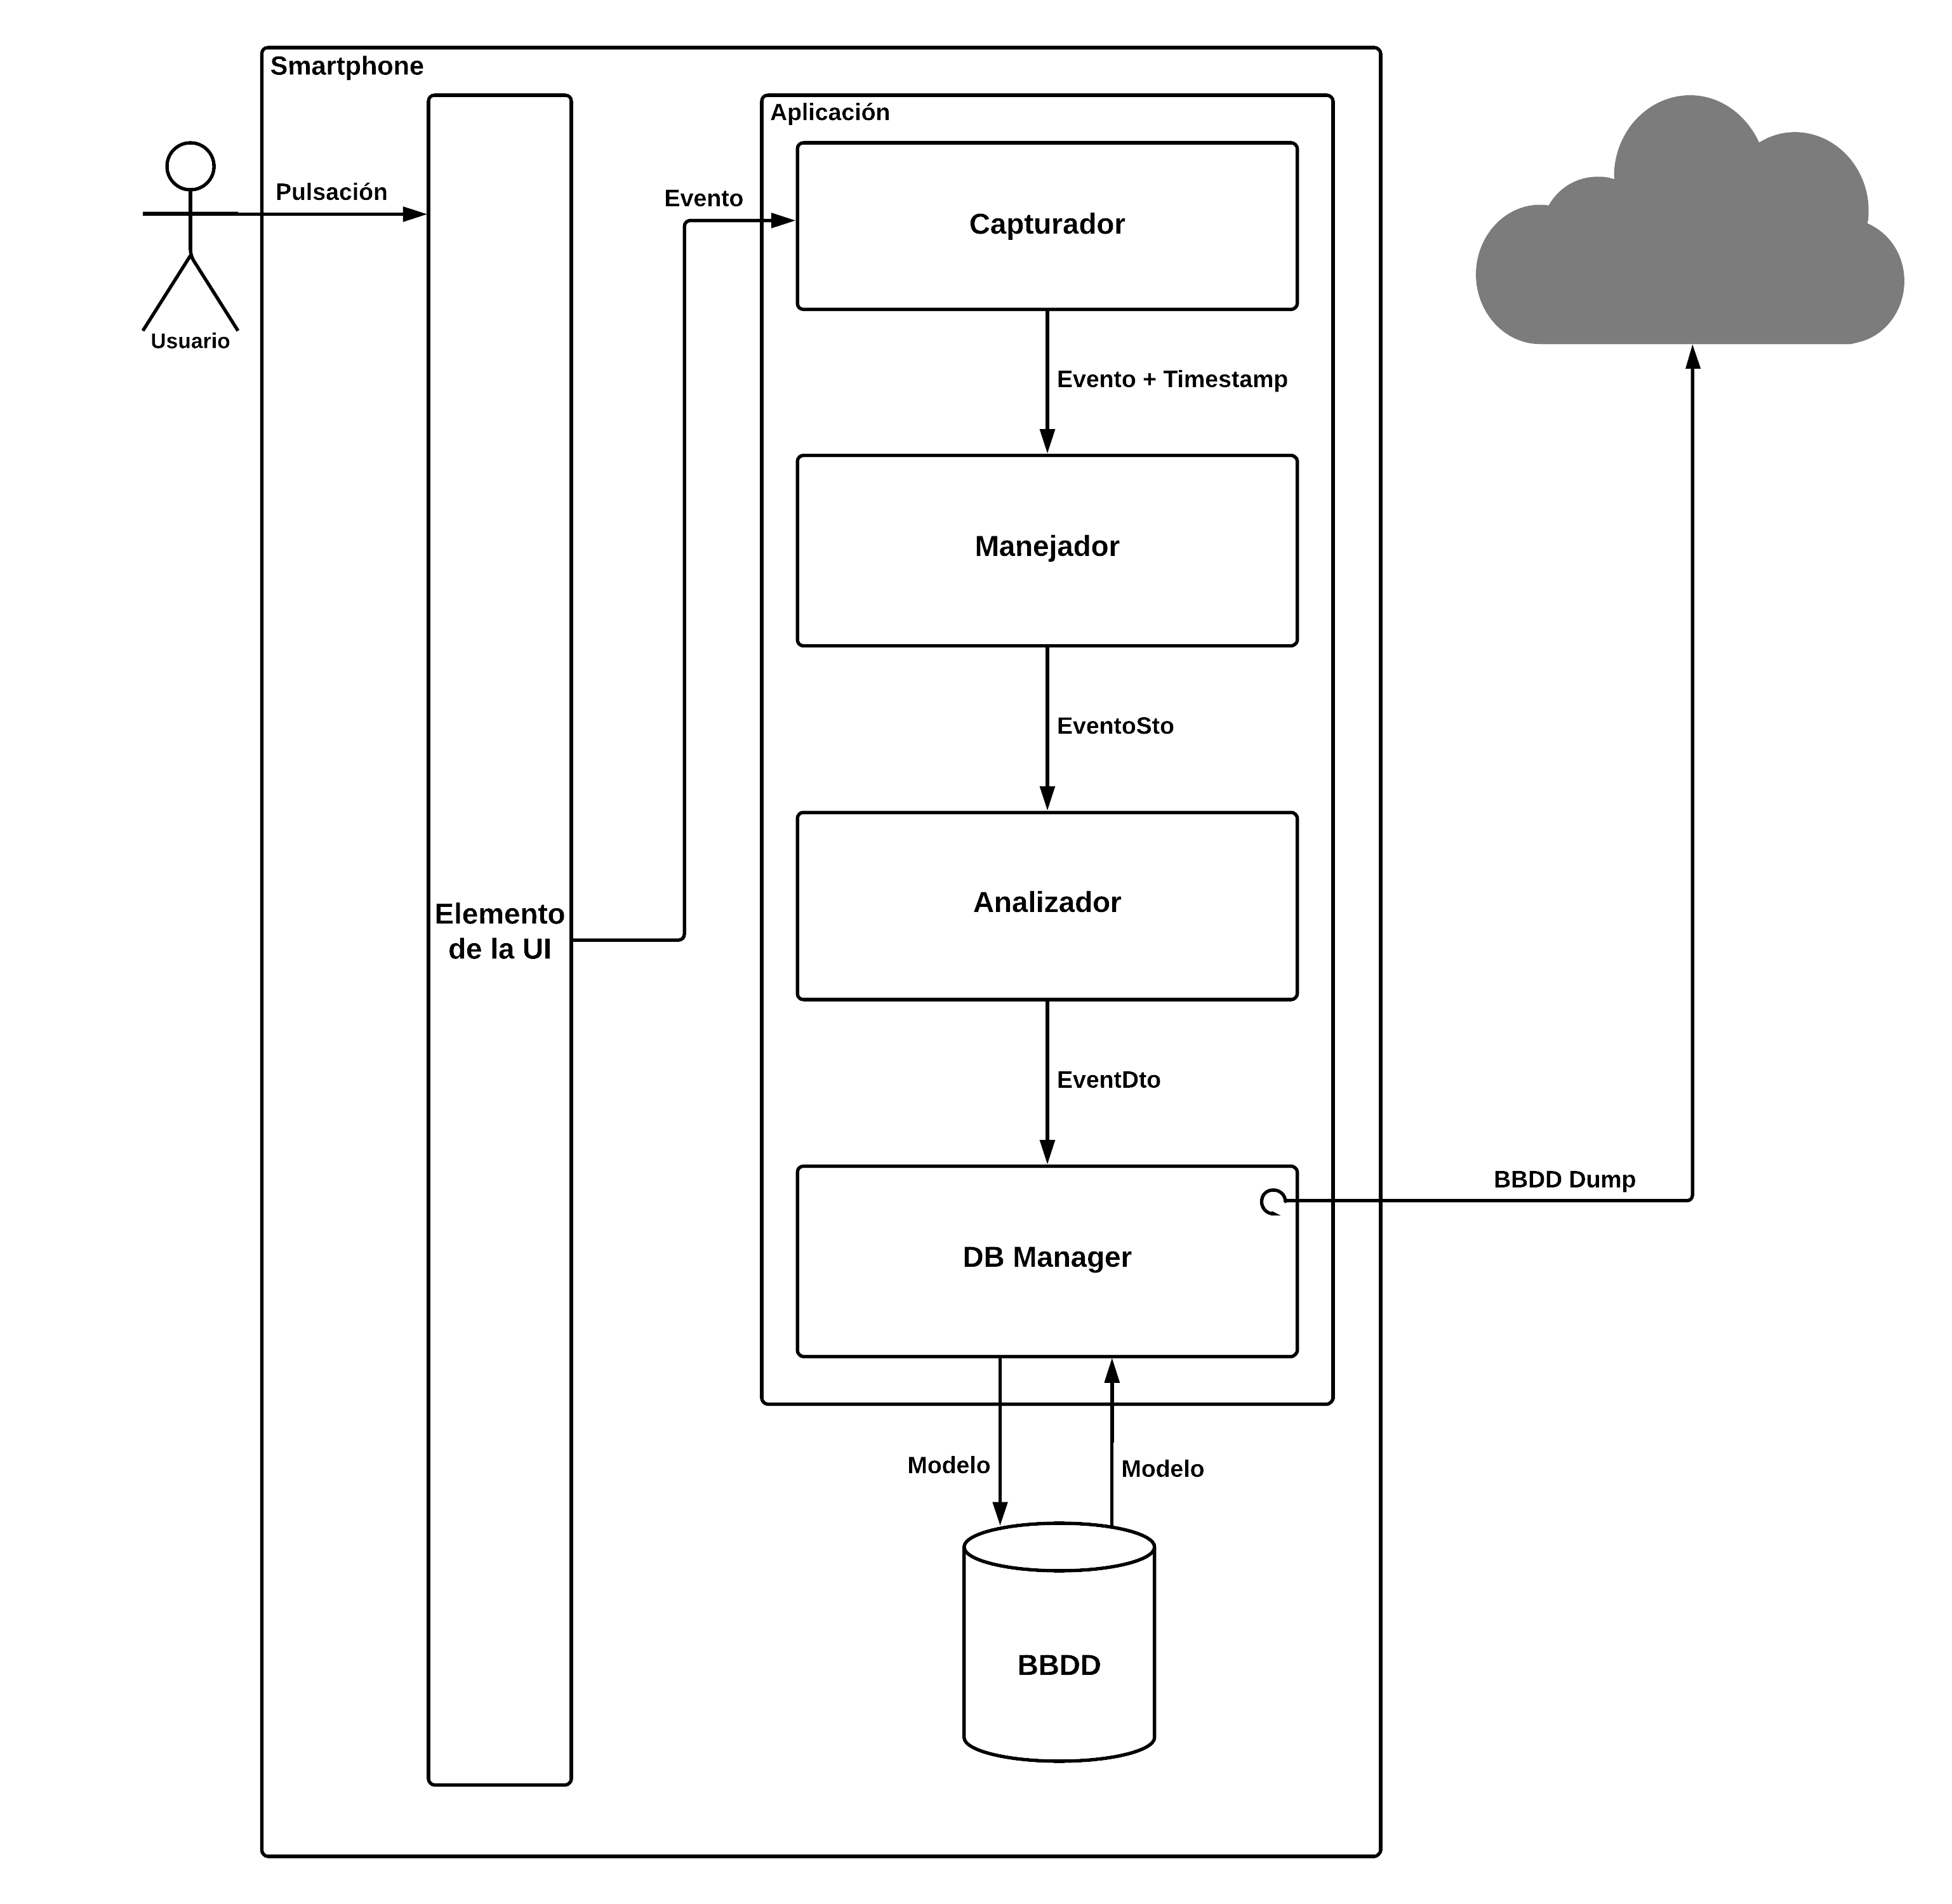
\includegraphics[width=1.2\textwidth]{pictures/architecture/highLevelArch01.png}
  \end{center}
  \caption[Arquitectura de alto nivel]{Arquitectura de alto nivel.}
    \label{fig:LandscapeFigure}
\end{figure}
\end{landscape}
%----------- P A N O R A M I C O -------------------------------------------------

\newpage
Vemos que el sistema se compone gracias a tres componentes fundamentales, por un lado el usuario, fuente de nuestros datos, el propio teléfono, en donde capturaremos la información, y un servidor en la nube que recibirá de forma periódica los datos recogidos por el teléfono y que permitirá además consultarlos. 
\newline
\newline
\subsection{Smartphone}
Vayamos por partes pues y analicemos cada grupo de componentes. Por un lado el \textbf{smarthphone} y el \textbf{usuario}. Dado que el smartphone es la interfaz de acceso del usuario a las funciones del teléfono y sus aplicaciones, será entonces aquí donde centremos nuestro sistema y donde estarán la mayor parte de sus componentes, al menos todos los relacionados con la captura de información. 
\newline
\newline
Este proceso de captura se detalla en el siguiente fragmento de la arquitectura. 
 %%% ------ 
\begin{figure}[hbt]
  \begin{center} \setlength{\unitlength}{0.0105in}
     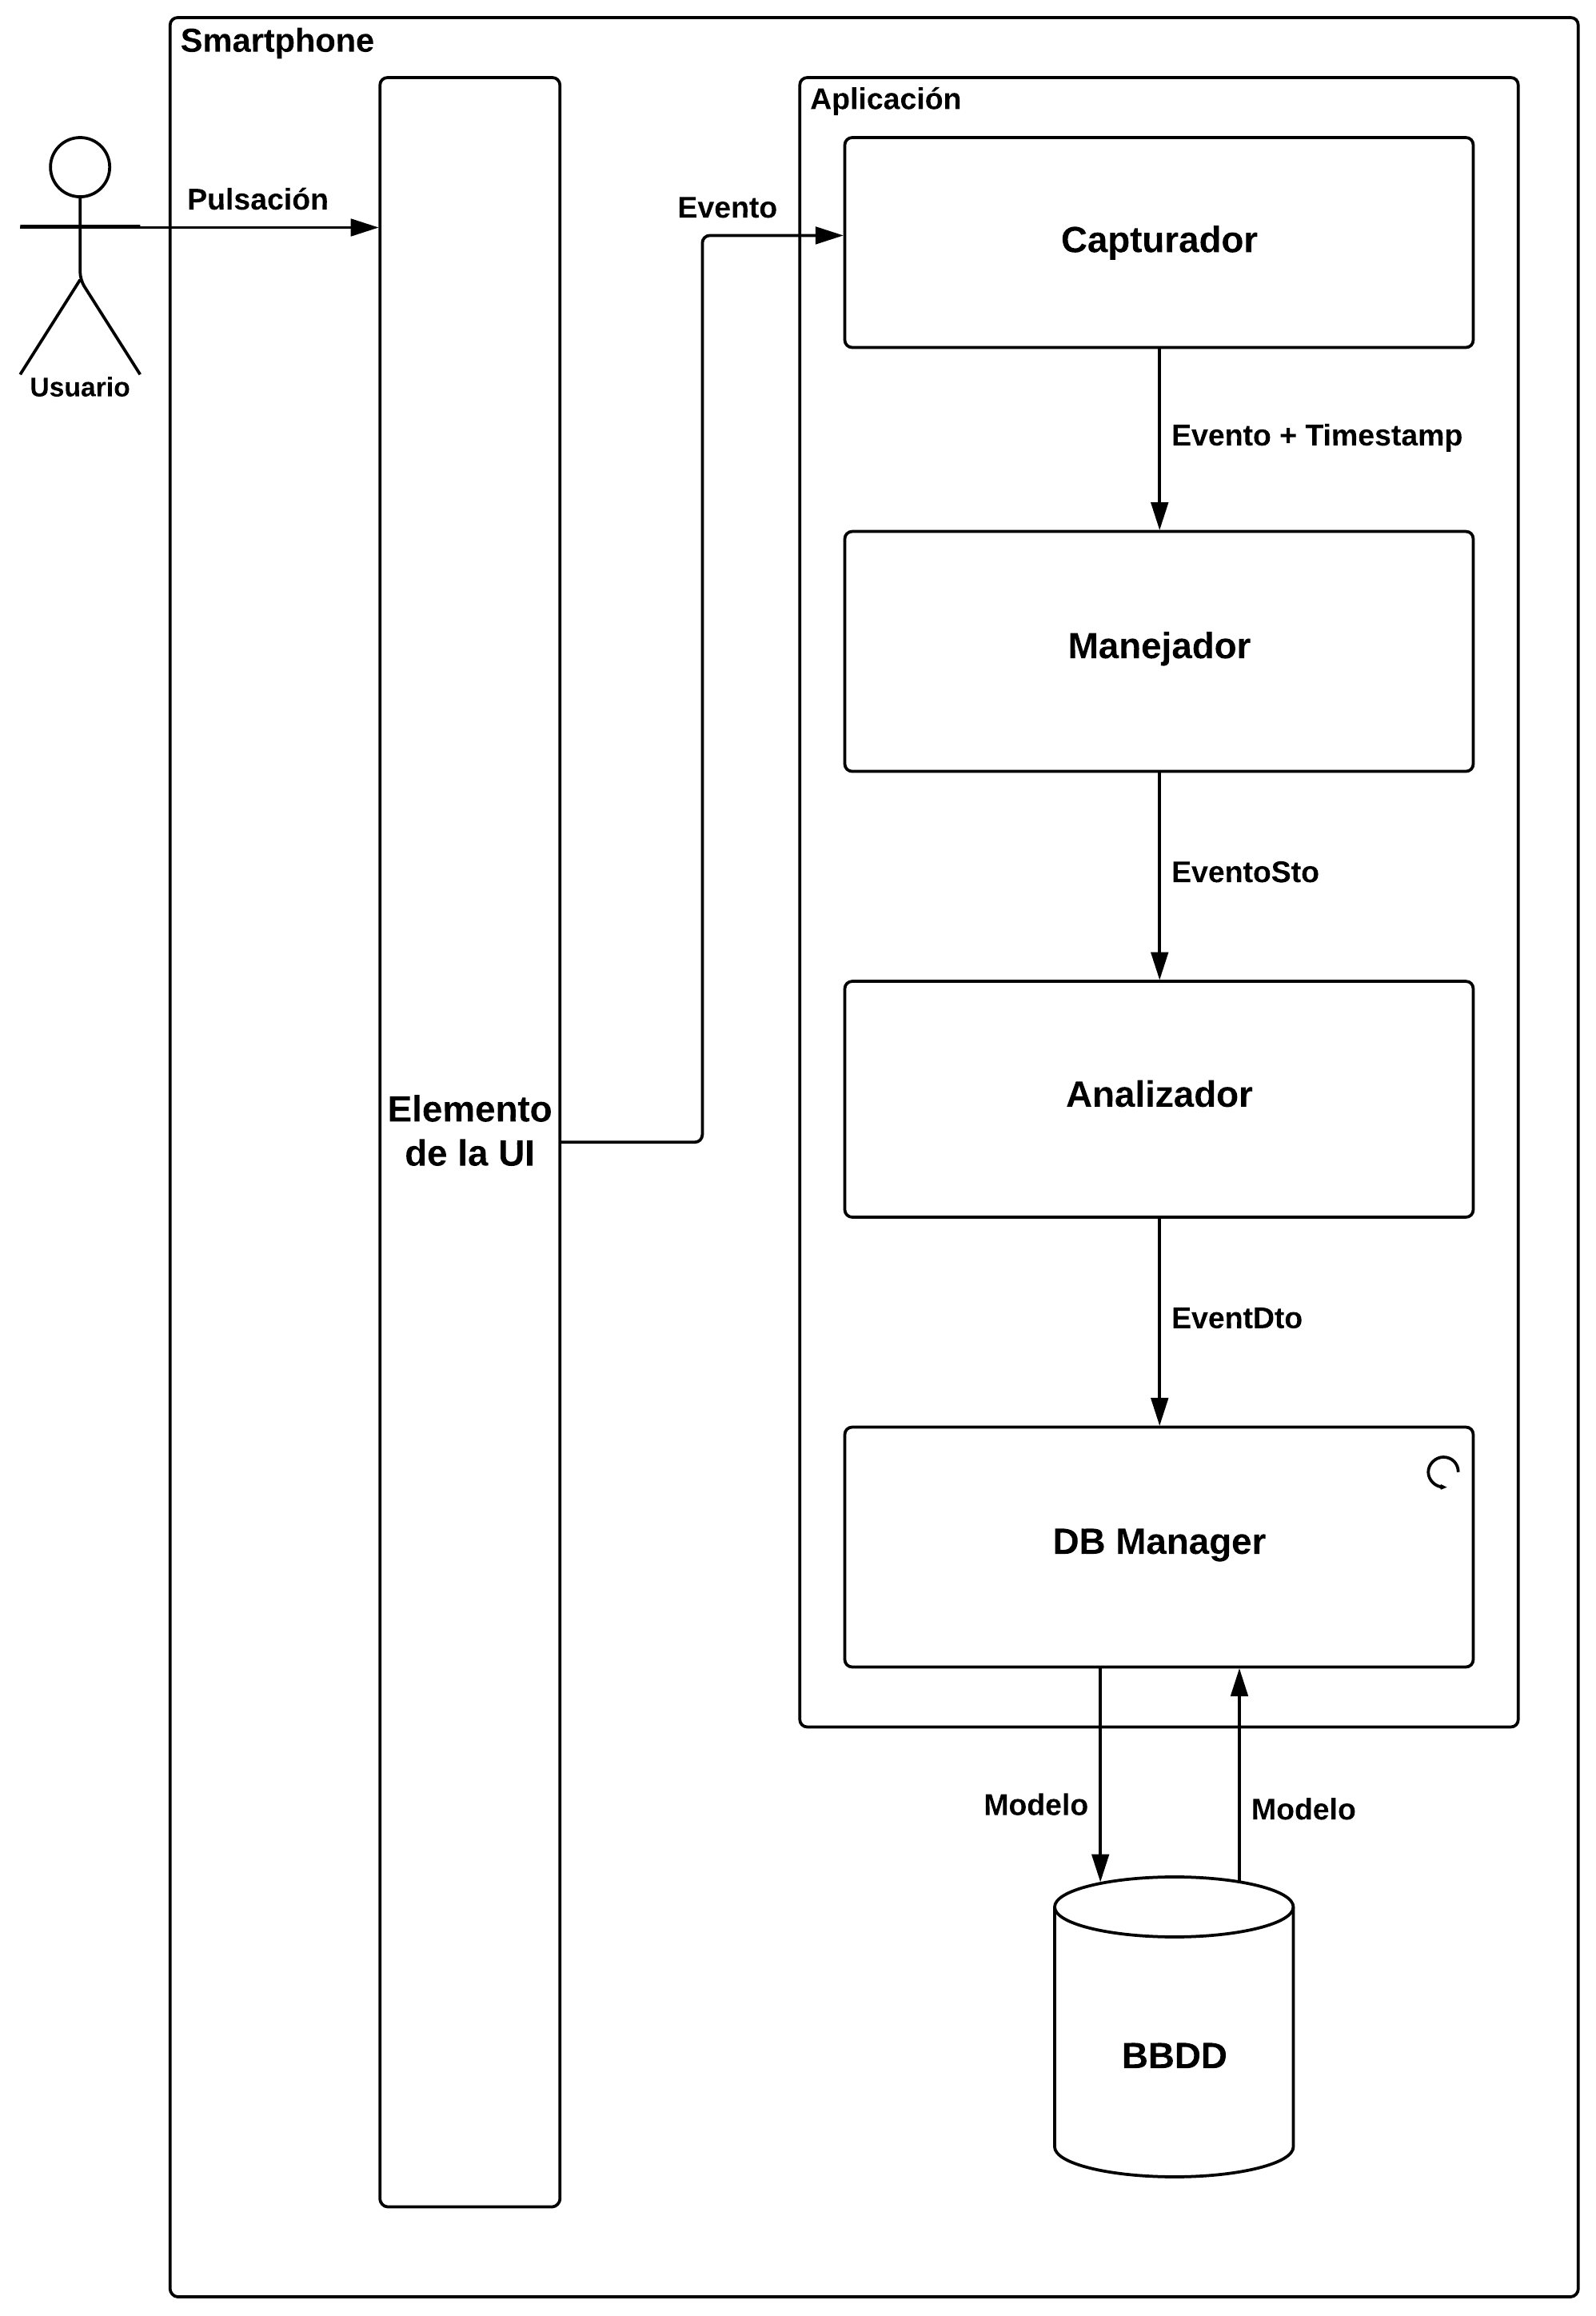
\includegraphics[width=0.5\textwidth]{pictures/architecture/highLevelArch02.png}
  \end{center}
  \caption[Arquitectura de alto nivel. Smartphone]{Arquitectura de alto nivel. Detalle de la parte móvil.}
\end{figure}
%%% ------
Toda la arquitectura parte del usuario, el cual interactúa con su teléfono mediante pulsaciones en la pantalla, que son recogidas por aplicaciones que le devuelven información al usuario mediante esa misma pantalla. Será entonces esta interfaz de usuario lo que nuestro sistema deberá escuchar y capturar. Por lo tanto tendremos una aplicación que recibirá las pulsaciones en los elementos de la interfaz del usuario (UI) bajo la forma de eventos. 
\newline
\newline
Vamos a desglosarla por cada elemento, viendo antes de cada componente la unidad de datos que va a manejar.
\newline
\newline
\subsubsection{Evento}
Estamos ante la información de entrada única y por tanto fundamental del sistema. Se trata de una unidad de datos compleja y sin estructurar. 
\newline
\newline
Los genera el sistema cada vez que ocurre un cambio notable en la pantalla, y su propósito es dar el mayor feedback posible del usuario. 
\newline
\newline
Muchas veces esta información no surge en el instante en el que se produce el evento, que no deja de ser una instantánea de la pantalla en ese momento, si no que se necesita un contexto, que lo aporta la relación que existe entre los eventos al estar asociados a través de un árbol, representando la vista que está viendo el usuario. 
\newline
\newline
Es por tanto, una unidad de datos muy cruda y desestructurada a la que hay que extraer el significado en su procesamiento en las capas inferiores. Por tanto este evento será producido por el sistema y la fuente de entrada del nuestro, a través del \textbf{capturador}.
\subsubsection{Capturador}
Se trata de un proceso que está siempre escuchando la aparición de nuevos eventos, con el objetivo de capturarlos y pasárselos al siguiente nivel de la arquitectura, el \textbf{manejador}. Su carga de trabajo realmente será poca, y consistirá en informar al manejador pasándole el evento junto al instante temporal en el que fué generado. 
\newline
\newline
Por lo tanto el capturador recibe eventos y genera eventos junto a su marca temporal para que los consuma el siguiente nivel, manejador. 
\subsubsection{Evento + timestamp}
No consiste en una unidad de datos como tal, puesto que sólo consiste en una fecha y hora y el propio evento asociado a ellos. 
\subsubsection{Manejador}
Recibe un evento y su marca horaria y debe encapsularlo para que el nivel inferior lo analice, es por tanto el nexo de unión entre los datos en bruto y los datos refinados. 
\newline
\newline
Para ello, cuando reciba el evento, en primer lugar lo encapsula junto a su marca horaria en un objeto que hemos llamado Sto. Simple Transfer Object. 
\newline
\newline
Una vez encapsulado, consulta la aplicación fuente del evento, es decír, la aplicación que lo generó, que nos permite establecer nuestro primer filtro y discernir si se trata de gmail, telegram, facebook... etc. 
\newline
\newline
En función de esto, se llamará a una implementación del analizador u otra, puesto que cada aplicación sigue su propio flujo lógico. Por ello se le comunica un Sto con la información fundamental que necesita. 
\subsubsection{Sto}
Es la unidad de datos empleado para comunicar el \textbf{manejador} con el \textbf{analizador}, se trata de una unidad de datos cuyo objetivo es encapsular la información en unidades contenidas y controladas. Será consumido por en analizador a través de la consulta de su evento y su marca horaria, siendo esta última fundamental para aportar el contexto necesario por el analizador. 
\subsubsection{Analizador}
Recibe los citados Stos, objetos sencillos, del manejador, para tratarlos, procesarlos y extraer su significao. 
\newline
\newline
Este procesamiento consisitirá en analizar, en base al modelo correspondiente, el patrón de llegada de los datos y en base a su contenido y el de eventos antecesores y sucesores, aportarle un contexto. Gracias a este modelo construiremos Dtos completos que representarán una unidad de información completa acerca del uso de la app.
\subsubsection{Dto}
Dtos, Data Transfer Objects, será la unidad última de información que genere nuestro sistema, representado así la información completa del usuario, es decir, uno de estos dtos contiene en su interior la interacción completa del usuario con cualquier servicio que le ofrezca el teléfono. 
\newline
\newline
Será por tanto contenido semántico de esta interacción, siendo por ejemplo, un dto una conversación mantenida por whatsapp con un contacto durante el intervalo de tiempo en el que estuvo activa, una búsqueda en el navegador... en resumen cualquier interacción, contextuada, del usuario con cualquiera de las apps que vamos a monitorizar. 
\newline
\newline 
Una vez estos Dtos están listos se les pasa al DB Manager. 
\subsubsection{DB Manager}
Capa encargada de la persistencia de los datos que le pasa el analizador. El manager los convierte en modelos para su almacenamiento en una base de datos local. 
\newline 
\newline 
En este manager recae una tarea también fundamental para el sistema, puesto que debe realizar un volcado periódico la base de datos a un servidor remoto para su seguridad y almacenamiento para posibles usos. 
\newpage
\subsection{Servidor Remoto}
En este apartado analizaremos la arquitectura del entorno remoto planteado por la arquitectura. Consiste en un servicio en la nube que acepta el volcado que realiza la base de datos del teléfono cada poco tiempo y permite además visualizar los datos allí vertidos. 
 %%% ------ 
\begin{figure}[hbt]
  \begin{center} \setlength{\unitlength}{0.0105in}
     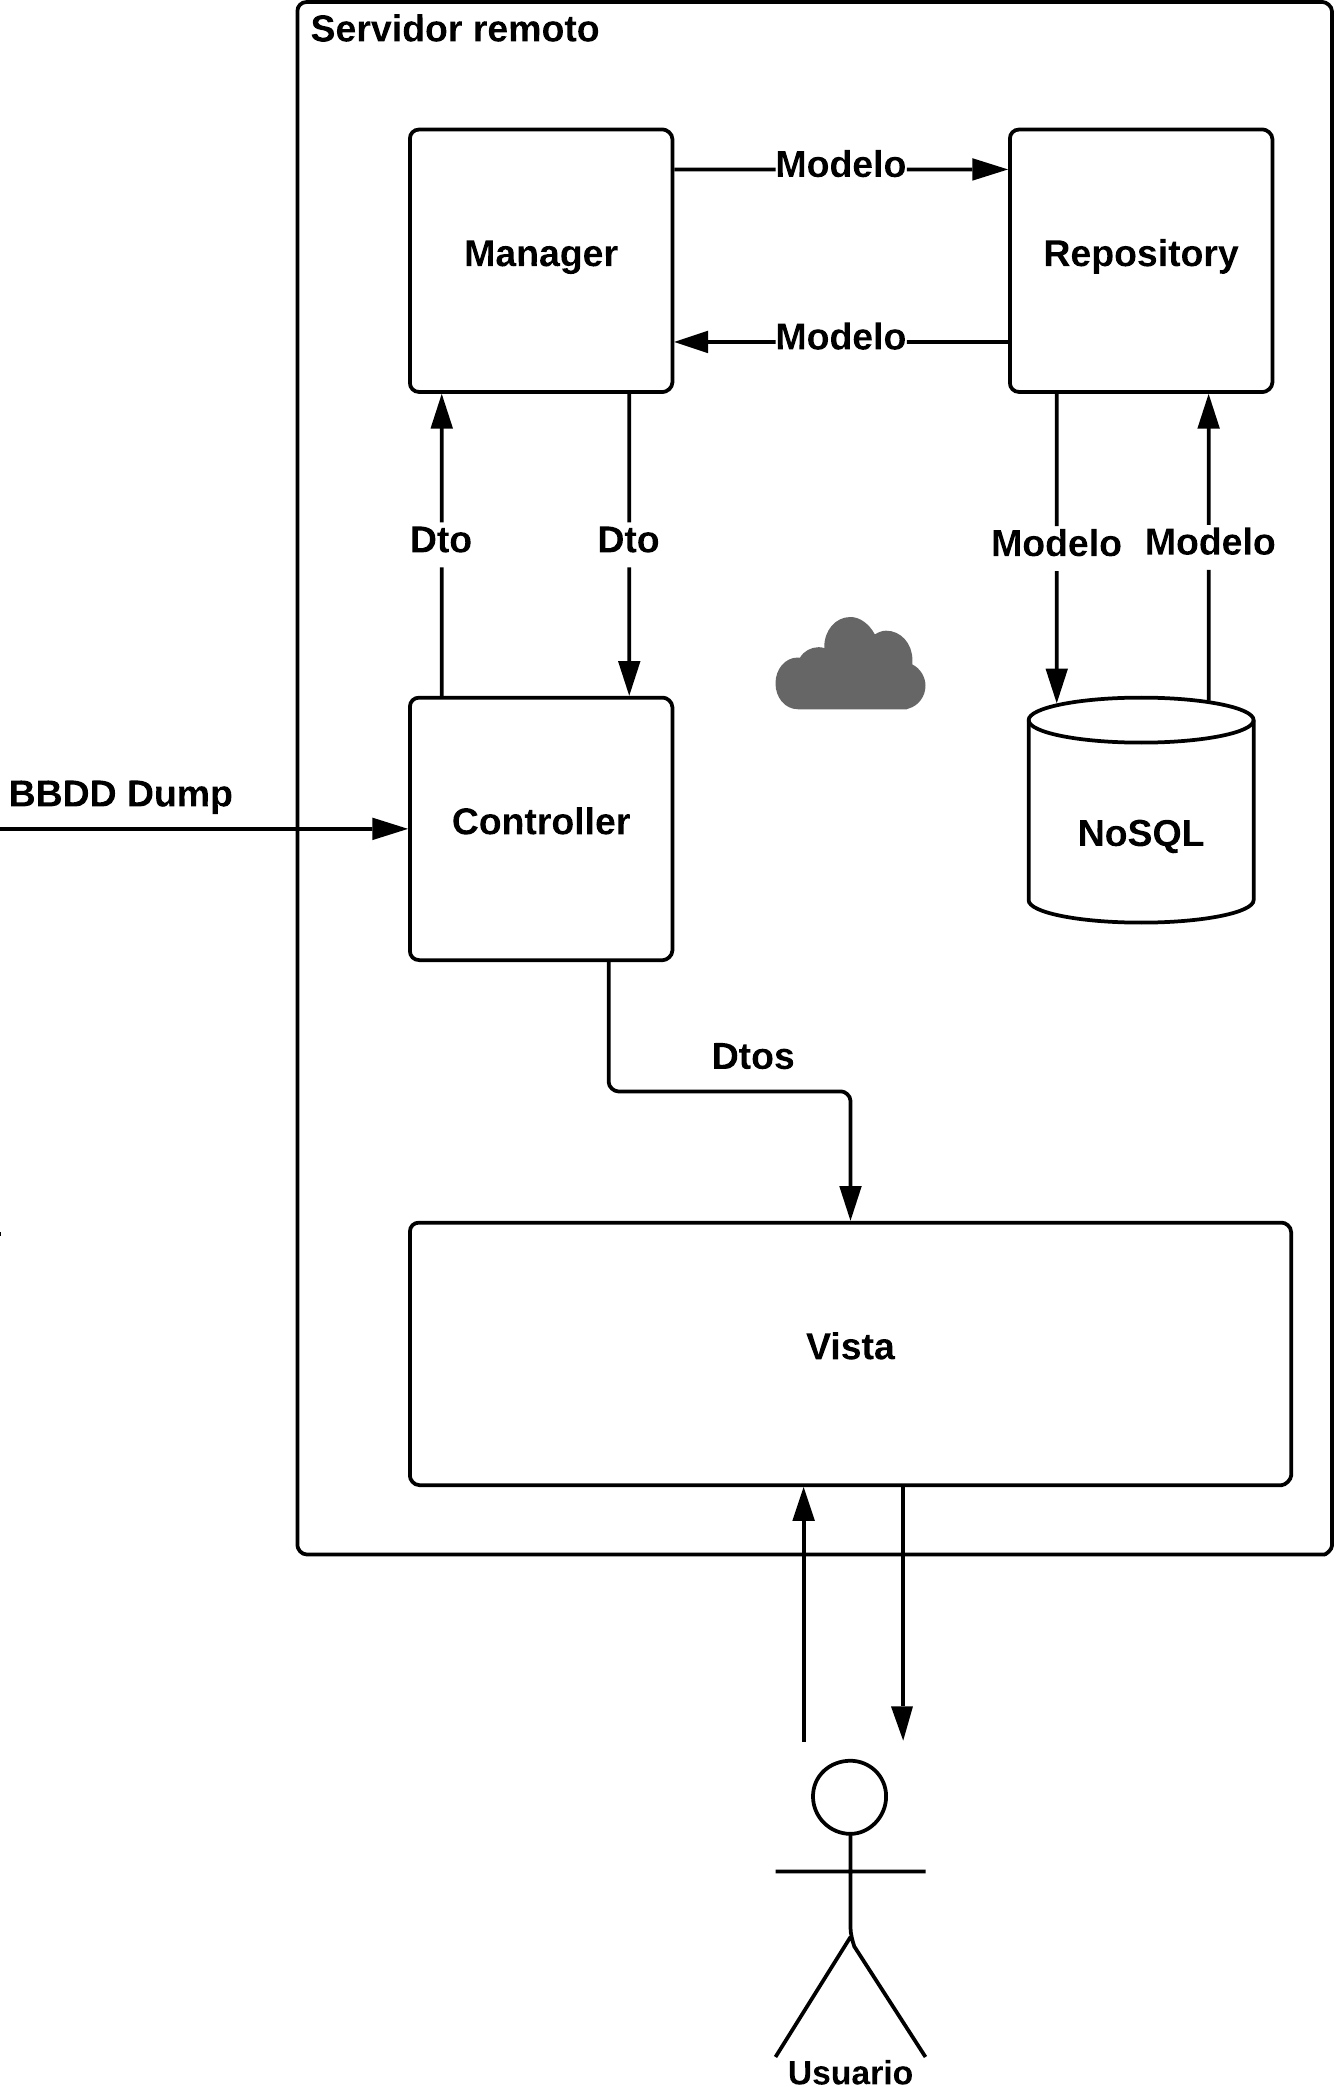
\includegraphics[width=0.5\textwidth]{pictures/architecture/highLevelArch03.png}
  \end{center}
  \caption[Arquitectura de alto nivel. Cloud]{Arquitectura de alto nivel. Detalle del entorno cloud}
\end{figure}
%%% ------
Estamos, por lo tanto, ante una típica arquitectura de servicios web, donde tenemos un controlador, encargado de atender los puntos de entrada de la API, un Manager que realiza las tareas de conversión de objetos y la lógica de negocio, el Repositorio, encargado trabajar contra la base de datos, una base de datos NoSQL y una Vista, 	que nos permite visualizar los datos almacenados. 
\subsubsection{Controller}
Proporciona la interfaz de entrada de la API a través de solicitudes HTTP, así, contaremos con un único método de entrada que aceptará datos en formato JSON, con el contenido en bloques de la base de datos del teléfono, así como los endpoints necesarios para la vista. 
\newline
\newline
Este controller extraerá los datos del json y los convertirá a Dtos, pasándoselos a su vez al manager para que realice la comunicación con las capas inferiores. 
\subsubsection{Manager}
Se encarga de transformar los dtos aportados por el controller en modelos que acepte la base de datos, así como realizar la operación inversa y convertir los datos de la base de datos en Dtos de forma que puedan ser invocados por el controlador y ser devueltos a la vista. 
\newline
\newline
Será por tanto el elemento del entorno cloud donde se depositará toda la lógica de negocio, transformaciones de objetos, mezclados, etc. 
\subsubsection{Repository}
Capa más próxima a la base de datos, nos ofrecerá un sistema de comunicación del resto de la plataforma con la base de datos, siendo este su único punto de entrada, donde manejaremos modelos acordes al esquema de los documentos almacenados en la DB NoSQL. 
\subsubsection{DB NoSQL}
Se trata de nuestra base de datos en la nube, se opta por un sistema NoSQL debido al gran volumen de datos que vamos a manejar. Con el crecimiento de estos datos, surge la necesidad de proporcionar información procesada a partir de grandes volúmenes de datos que tienen unas estructuras horizontales más o menos similares, y este es justo el escenario donde el uso de NoSQL nos brinda la mejor solución. 
\subsubsection{Vista}
Punto de salida de nuestra plataforma cloud, proporcionando así una interfaz de consulta de los datos almacenados, generados por la aplicación. \\
\newpage 
\section{Diagrama de secuencia}
Con el fin de explicar cual es el flujo que recorren los datos y las operaciones que realiza cada componente así como los mensajes que se intercambian entre ellos, se incluye a continuación un diagrama de secuencia que describe el ciclo de vida de un evento desde el instante en el que se dispara hasta el momento en el que se almacena su información. 
\begin{landscape}
\begin{figure}[htb]
  \begin{center}
     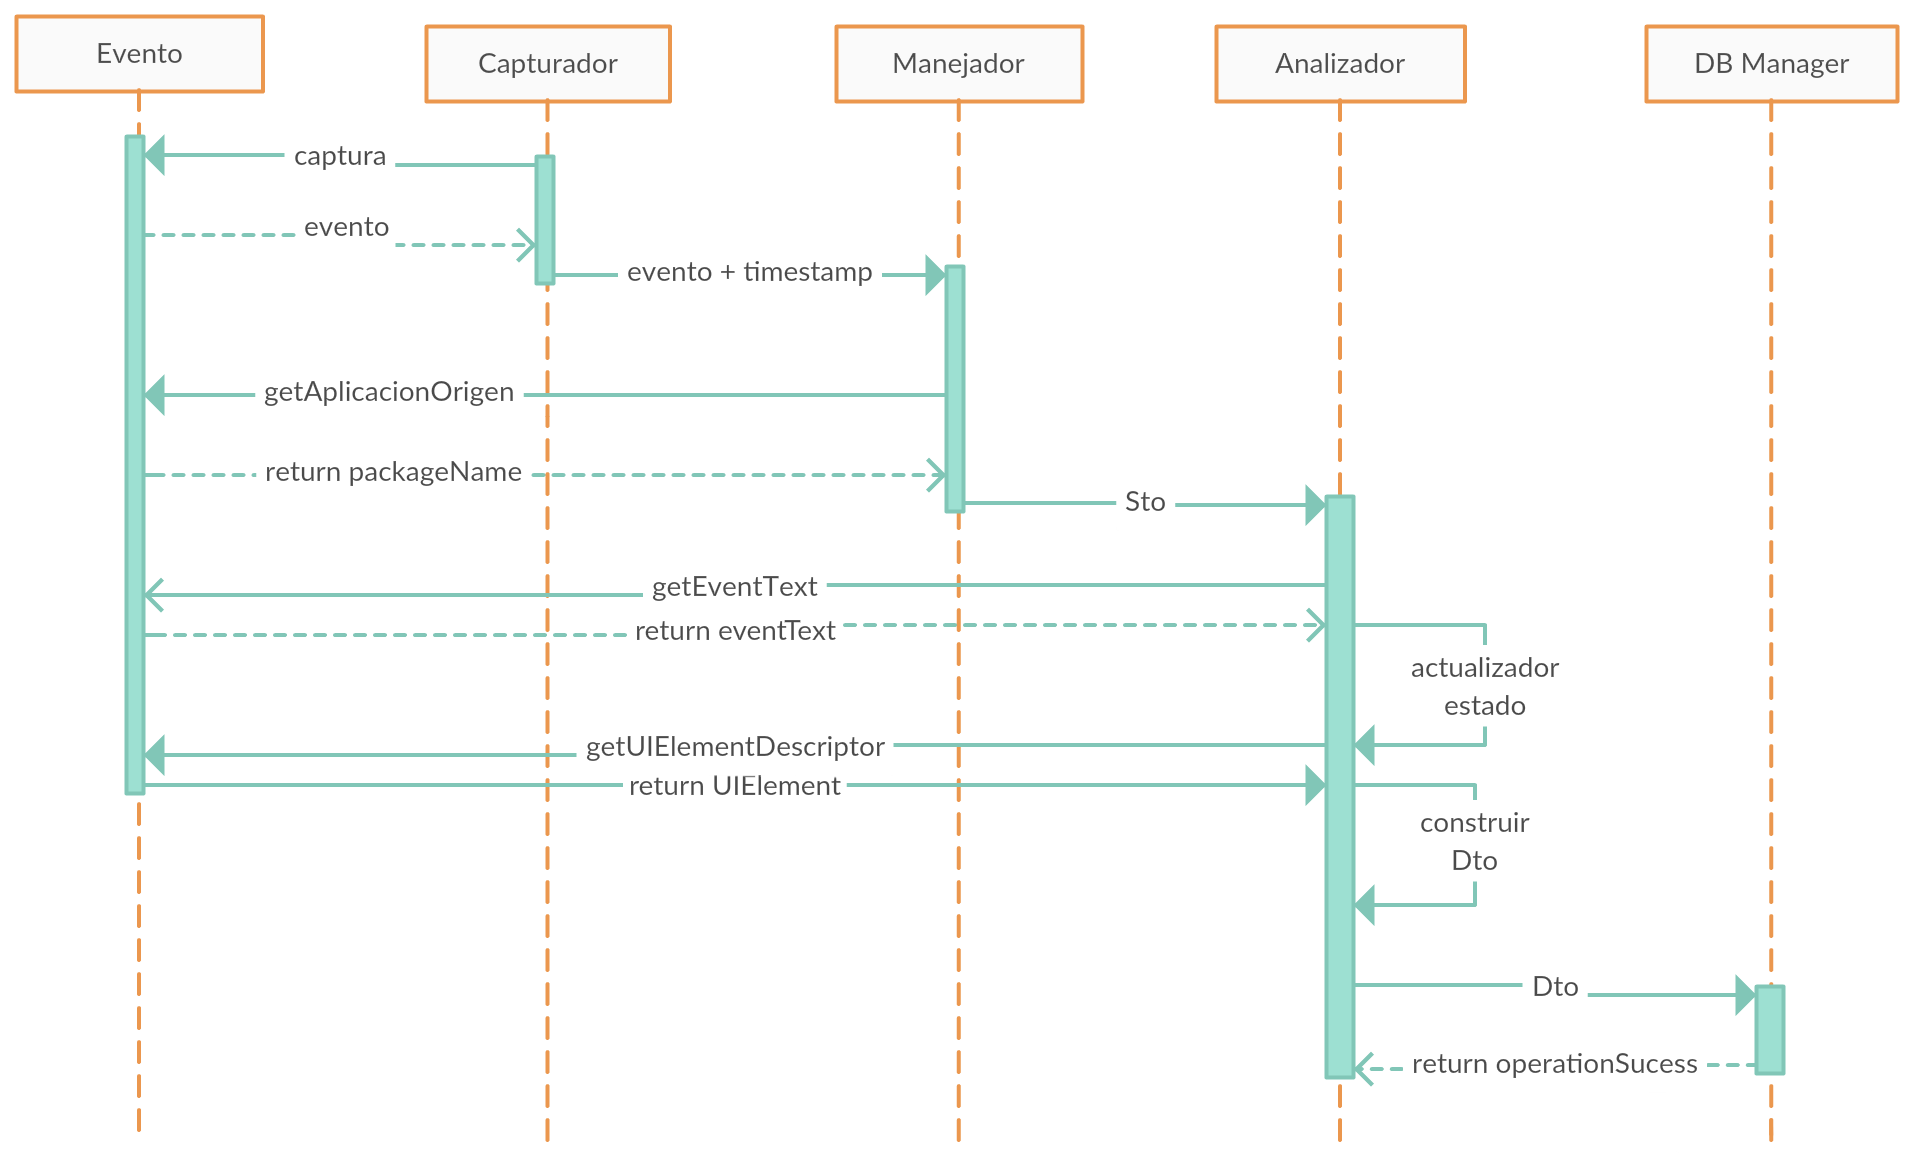
\includegraphics[width=1.5\textwidth]{pictures/secuencediagrams/diagrama_seq_flujo.png}
  \end{center}
  \caption[Diagrama de secuencia]{Diagrama de secuencia habitual del sistema.}
    \label{fig:LandscapeFigure}
\end{figure}
\end{landscape}


% -------------- %
% --- DISEÑO --- %
% -------------- % 
\chapter{Diseño}
En este capítulo se detalla el resultado de las sucesivas iteraciones sobre la etapa de diseño. A partir de los requisitos se ha estudiado el problema y planteado una arquitectura que nos permitirá guiar la implementación de los casos de uso. Se pretende obtener una arquitectura limpia y organizada de manera que permita la mantenibilidad del proyecto y una modificación mínima y eficaz. 
\newpage
\section{Arquitectura}
A la hora de plantear nuestra arquitectura el primer paso es conocer la propia arquitectura de Android.
\newline
\newline
Si nos fijamos en la siguiente figura vemos como Android se asienta en una modificación del Kernel de Linux sobre el que se van abstrayendo capas en las que cada una emplea los servicios que provee la capa inmediatamente inferior. 
%%% ------ 
\begin{figure}[H]
	\begin{center}
		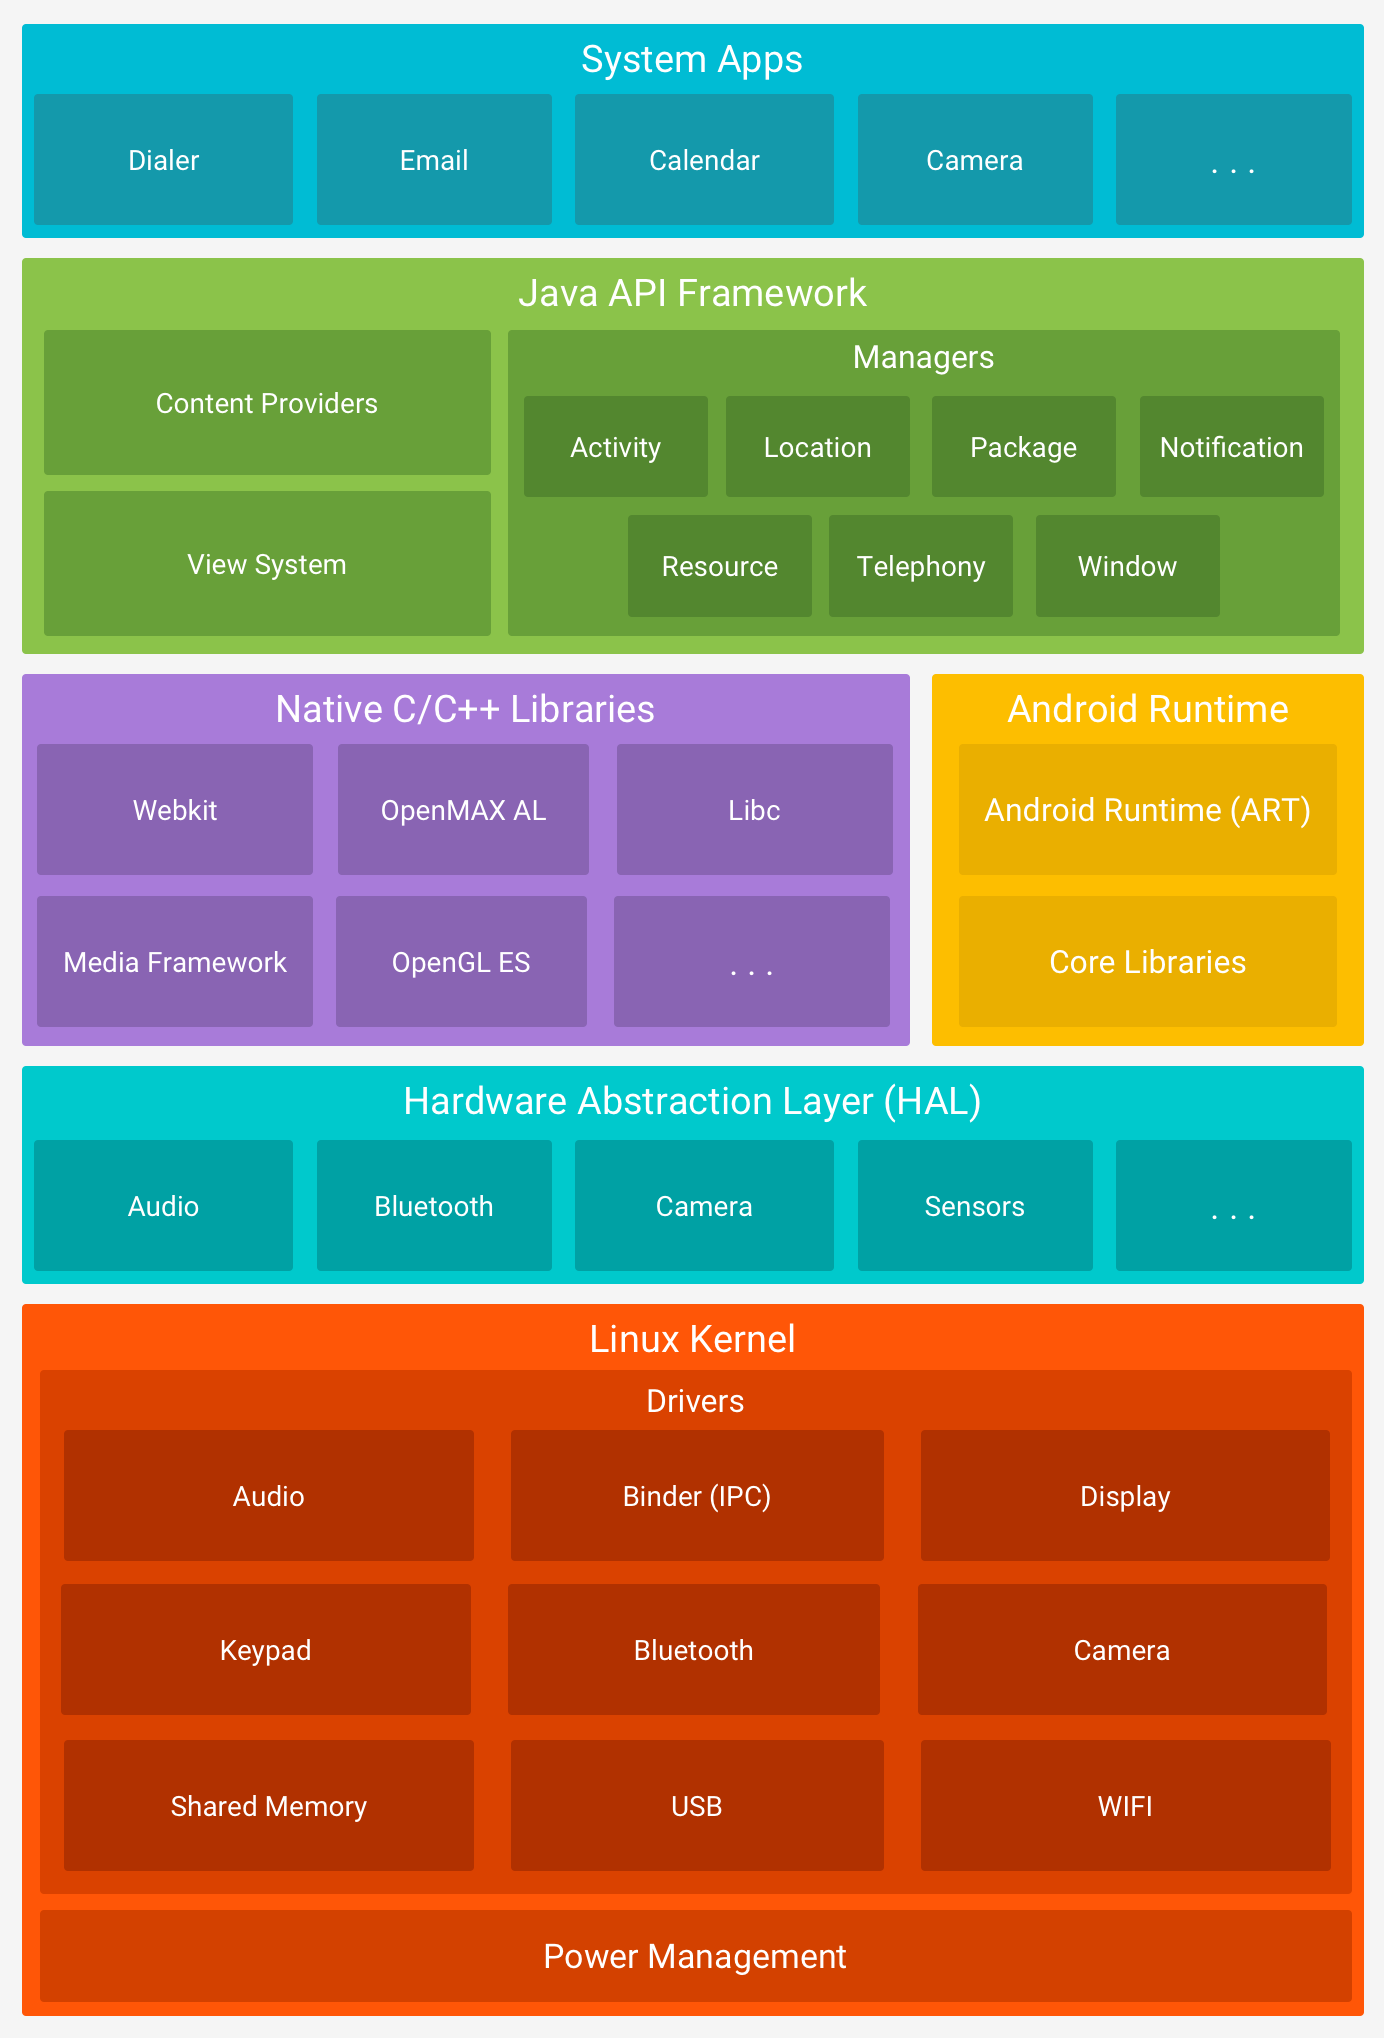
\includegraphics[scale=0.15]{pictures/architecture/android_stack.png} % include ./img/imagen.[pdf|png|jgp] si es pdflatex o ./img/imagen.eps si es latex
	\end{center}
	\caption[Android stack]{Arquitectura por capas de Android.}
\end{figure}
%%% ------
Así, como base de la arquitectura tenemos una modificación del Kernel de Linux sobre la cual se implementa una segunda capa, de abstracción del hardware, que será la encargada de manejar y comunicarse con los periféricos del teléfono. Entendemos por periféricos lo habitual en estos entornos; sensores, antenas, emisores radio...). Sobre estas dos capas, que permiten una interfaz de acceso al dispositivo Hardware, tenemos las librerías de bajo nivel y el entorno de ejecución de android. 
\newline \newline
Si avanzamos un poco más vemos que en las dos últimas capas están relacionadas con una API Java que permite al programador implementar aplicaciones, usando a través de la api, todo la anteriormente expuesto. 
\\
%%% ------ 
\begin{figure}[H]
	\begin{center}
		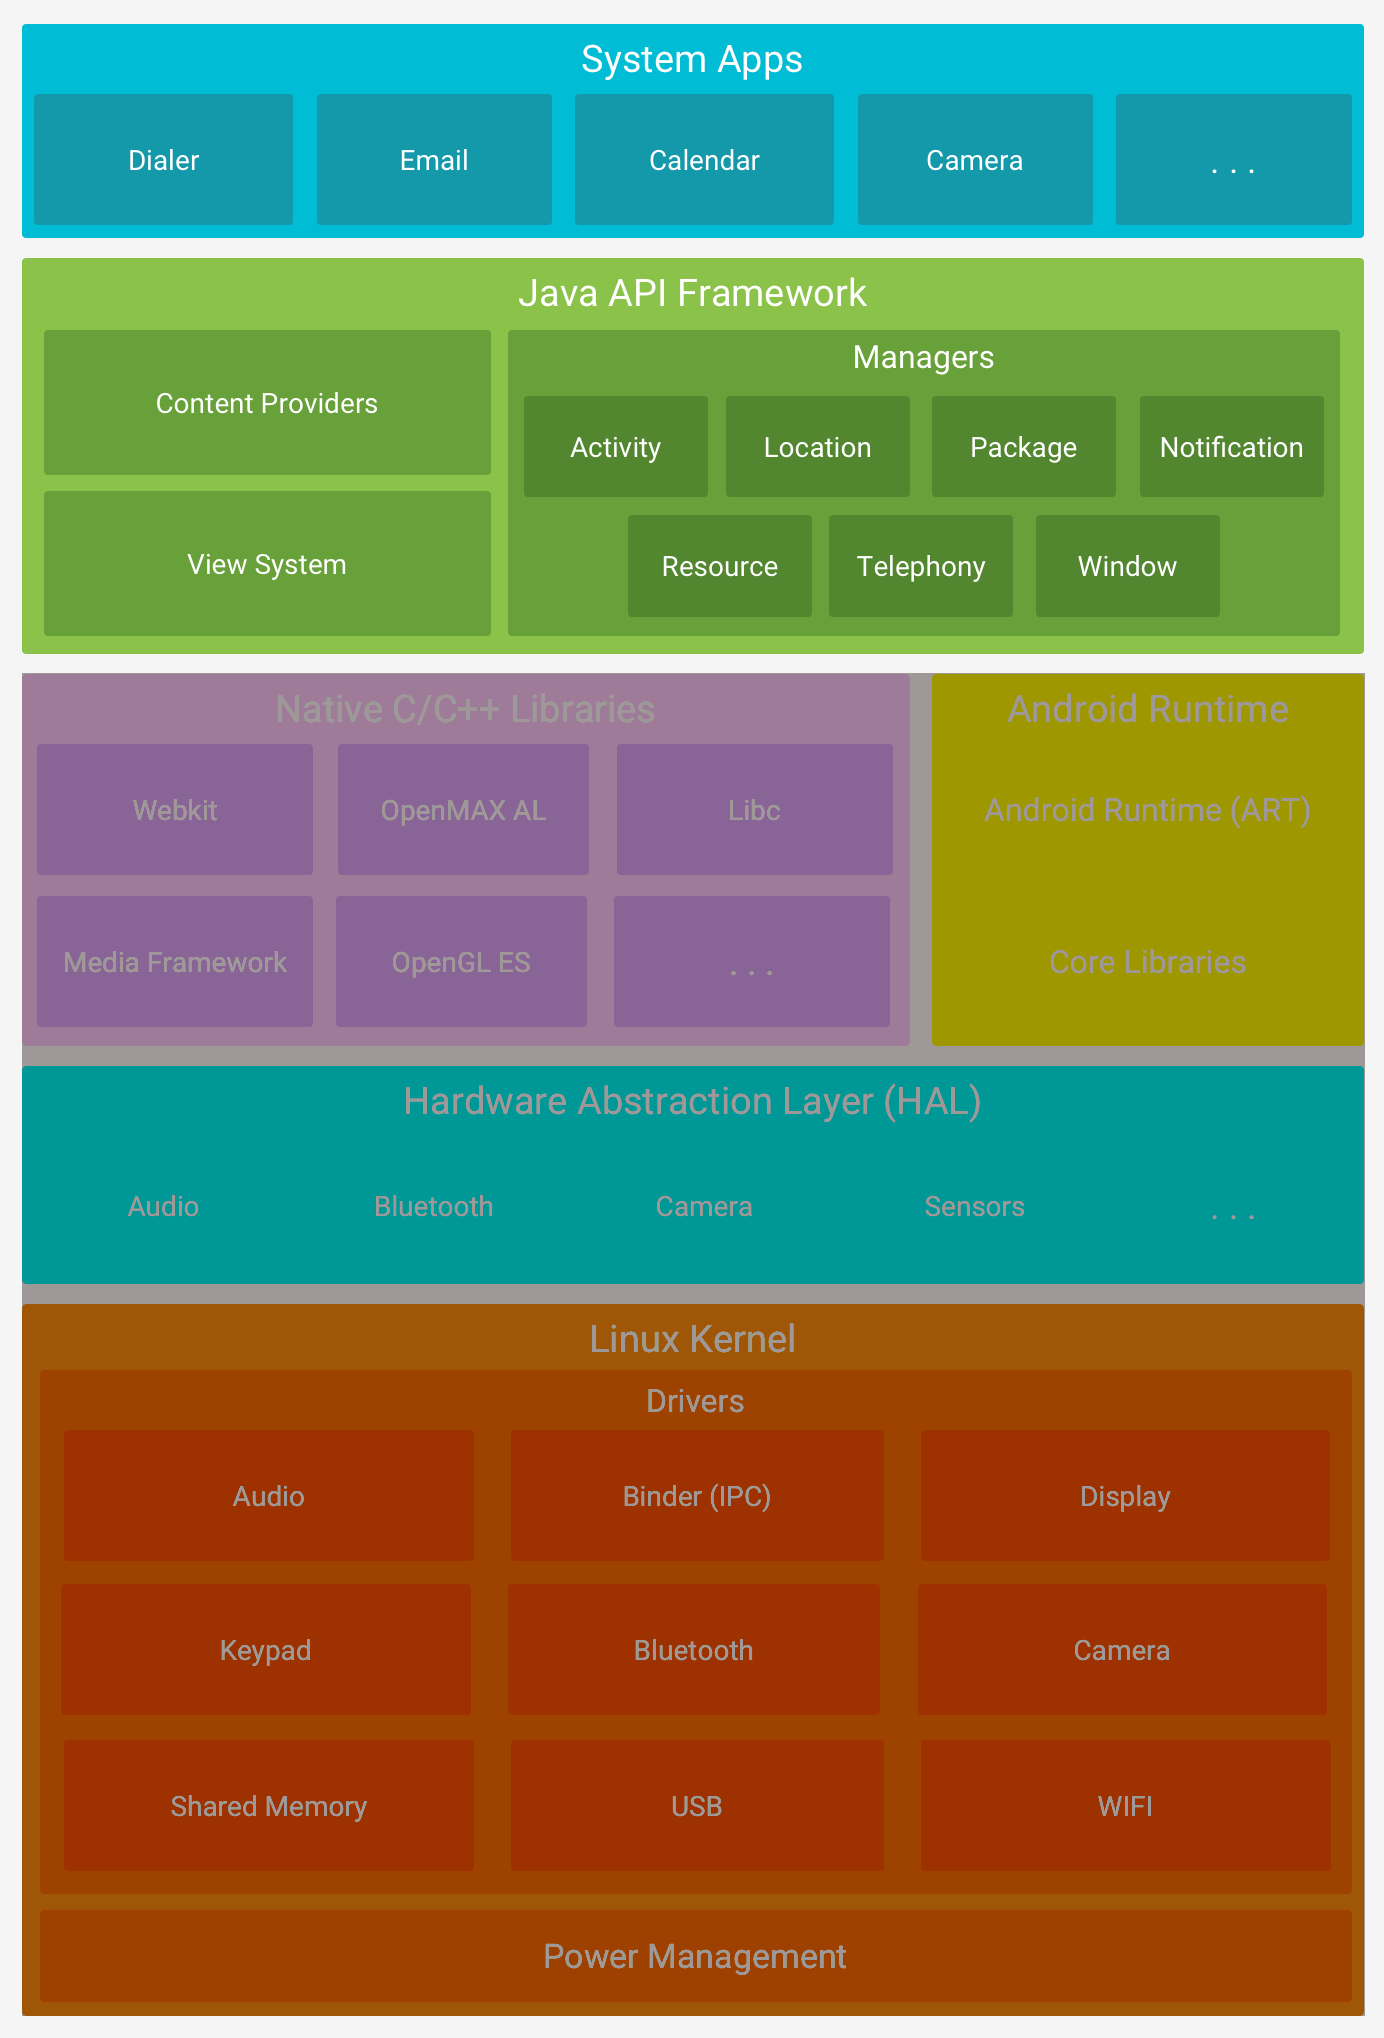
\includegraphics[scale=0.2]{pictures/architecture/android_stack_used.png} 
	\end{center}
	\caption[Detalle del Android Stack]{Márgenes del sistema}
\end{figure}
%%% ------
Estas dos últimas capas serán en las que se situará nuestra arquitectura. Además será conceptualmente parecida puesto que como hemos visto, Android dispone de un sistema organizado por capas, algo bastante lógica y habitual en los sistemas software, y nuestro objetivo por tanto debe ser separar funcionalidades y agruparlas bajo este patrón.
\newpage
\break
Teniendo este concepto claro, nos fijaremos en la publicación de Robert C. Martin, Clean Architecture, en la que se plantea el concepto de Arquitectura Limpia, sin ser más que una serie de condiciones que debe cumplir una arquitectura para que se la considere ”clean". Nos encontramos entonces con una serie de reglas, cuyo cumplimiento ayuda a diferenciar y dividir el software en capas, obteniendo además un software independiente de elementos externos (como la ui, frameworks y bases de datos), testeable y mantenible. 
\newline
\newline
En esta publicación nos encontramos con que una arquitectura debe partir de las entidades (entities). Estas entidades no son mas que las implementaciones sencillas de clases Java. 
\newline
\newline
Estas clases permitirán instanciar objetos que reprensentarán a los actores principales de la lógica de negocio. Por tanto POJOS (Plain Old Java Object) y Dtos (Data Transfer Objects) se verán incluidos en esta capa. 
%%% ------ 
\begin{figure}[H]
	\begin{center}
		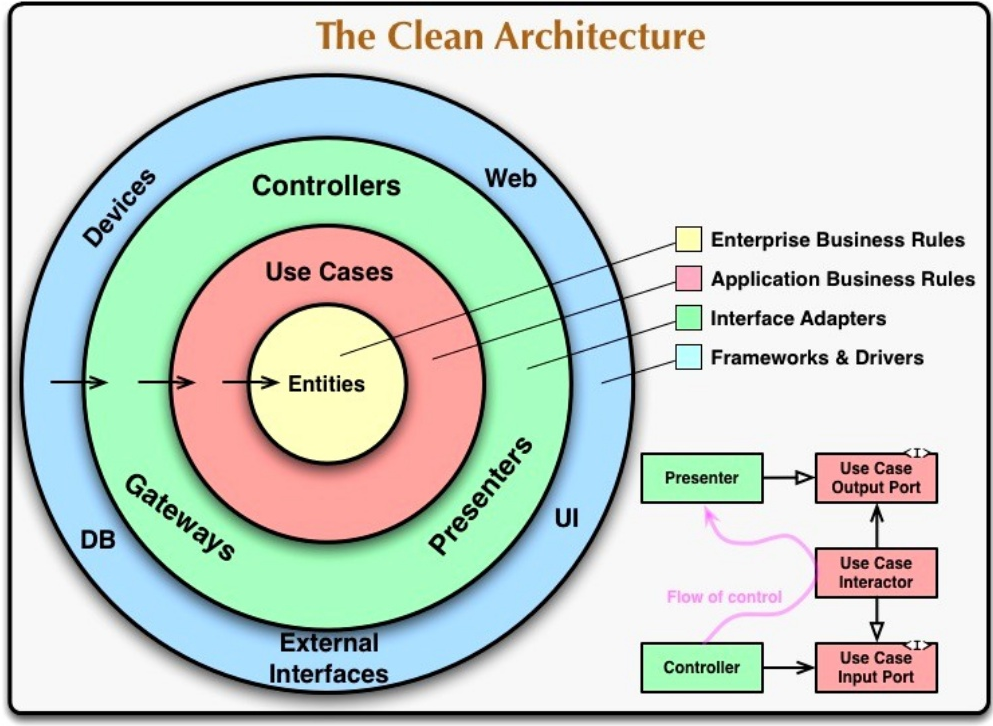
\includegraphics[scale=0.3]{pictures/architecture/android_architecture.png} 
	\end{center}
	\caption[Clean Architecture]{Arquitectura clean}
\end{figure}
%%% ------ 
Los casos de uso (use cases) están muy relacionados con las entidades, puesto que implementarán la lógica de negocio del sistema, puesto que deben orquestar y orientar todo el flujo de datos del sistema. 
\newline
\newline
La capa de los Interface Adapters realiza la conversión de los datos de manera que se puedan comunicar los niveles superiores con los casos de uso y entidades (en MVC corresponde a los Controladores, MVVP al presenter... etc). 
\newline
\newline
En la última capa y más externa, Frameworks and Drivers, residen las plataformas y herramientas externas, donde se incluye la interfaz de usuario, web... 
\newline
\newline
Si nos planteamos esto en los términos del proyecto, es decir, una aplicación que sea capaz de meterse en los servicios de accesibilidad que provee para capturar, procesar y extraer la  información de los eventos que se generan, deberemos abstraernos del problema y ser capaces de, a partir de una vista general del sistema inferir las capas que finalmente nos guiarán la implementación. 
\newline
\newline
Así pues, en primer lugar situar nuestro sistema dentro del stack tecnológico de Android citado al principio de esta sección. 
\newline
%%% ------ 
\begin{figure}[H]
	\begin{center}
		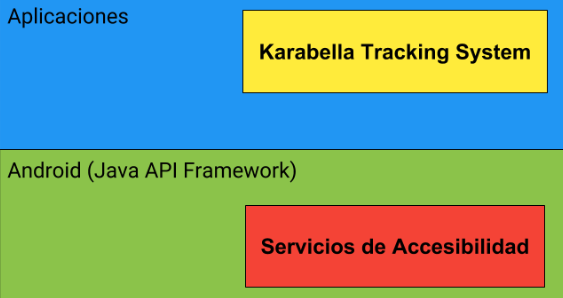
\includegraphics[scale=0.6]{pictures/architecture/arquitecturaGeneral01.png} 
	\end{center}
	\caption[Arquitectura dentro del android stack]{Arquitectura del sistema dentro del stack de Android.}
\end{figure}
Es natural esta clasificación puesto que el proyecto se basa en la implementación de los Servicios de Accesibilidad que Android dispone en de su API, gracias a mecanismos como la herencia y la implementación de interfaces. 
\newline \newline
Estos servicios de accesibilidad son la solución de Google para asistir y dar soportes a usuarios con diversidad funcional. Su naturaleza y comportamiento es lo que nos permite aprovechar estos servicios para obtener información de lo que hace el usuario. 
\newline \newline
Se comporta además como cualquier otro servicio de Android, (es decir, procesos ideados para correr en segundo plano con un ciclo de vida prolongado en el tiempo). Los Servicios de Accesibilidad se comportan al final como listeners de Eventos de Accesibilidad, que lanzados por el sistema. Estos Eventos de Accesibilidad son la entidad que manejan los servicios de accesibilidad. 
\newline \newline
Los eventos llevan consigo información sobre la interfaz de usuario, por ejemplo los eventos se lanza cuando entra en foco un elemento (con la descripción del elemento, botones, entradas de texto, nombres de ventanas...). Nuestra solución pasa por extraer la información de esos eventos y procesarla. 
\newline \newline
Dado que estos eventos pueden ser capturados por Eventos de Accesibilidad, nuestro sistema contará con un servicio que lo implemente y que realiza esta captura, este será un elemento fundamental en la arquitectura puesto que será la base sobre la que se asentarán el resto de elementos. 
\\
Así, en un primer vistazo, podemos ver la arquitectura usando un grano gordo del siguiente modo. 
%%% ------ 
\begin{figure}[H]
	\begin{center}
		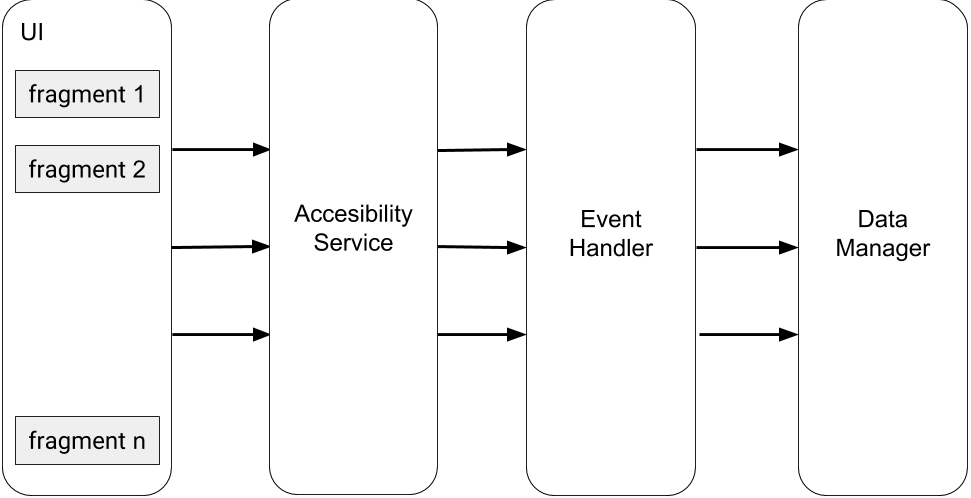
\includegraphics[scale=0.3]{pictures/architecture/arquitecturaGeneral02.png} 
	\end{center}
	\caption[Arquitectura general del sistema]{Arquitectura general del sistema}
\end{figure}
%%% ------ 
Donde la interfaz de usuario (UI) genera eventos de accesibilidad. Estos eventos, como ya se ha comentado, están asociados a cada acción que el usuario realiza con el teléfono sobre la interfaz. Será la implementación del evento de accesibilidad (Accesibility Service) el que nos permita capturarlos. 
\newline
\newline
Este servicio se encargará de capturar los eventos y mandarlos hacia el Manejador de Eventos (Event Handler), este manejador será el encargado de clasificar y procesar los eventos en función de la información que traigan consigo. 
\newline
\newline
Una vez que estos eventos pasen por el manejador, obtendremos como resultado una entidad lista para ser guardada en la base de datos. 
\newline
\newline
Profundicemos un poco más en como sería este manejador y como son los componentes que lo forman. 
\newline
\newline
Como estamos viendo, el servicio de accesibilidad (lo llamaremos simplemente servicio) recibe eventos de la interfaz y los envía al manejador, pero dado que los eventos se generan en gran cantidad y en momentos puntuales tendremos que manejar un caudal de información importante, la comunicación entre el servicio y el manejador se realizará a través de un bus que permitirá al servicio desatender los datos lo antes posible y desentenderse así de lo que ocurre con esos datos y como son tratados.
\newline
\newline
Este bus lo estará escuchando el manejador, que capturará los elementos para realizar un primer chequeo, y es que en función del nombre de la aplicación (más concretamente su package name), invocará a un \textit{Scraper} encargado de extraer la información relevante del evento que estamos manejando. 
\newline
\newline
Estos Scrapers son un concepto sacado del llamado \textit{Web Scraping}, técnica mediante la cual se transforman los datos sin estructura de la web en datos estructurados que pueden ser almacenados y analizados en una base de datos. 
\newline
\newline
Así pues, en nuestro sistema tendremos de tantos Scrapers como aplicaciones estemos monitorizando. Procesarán el evento de accesibilidad y lo encapsularán en una unidad de datos que será pasada a la capa de persistencia, formada por los Managers. Encargados de persistir en una base de datos local los datos generados por el sistema. 
\newline
\newline
Al final nuestra arquitectura a bajo nivel resulta en el siguiente diagrama. 
%%% ------ 
\begin{figure}[H]
		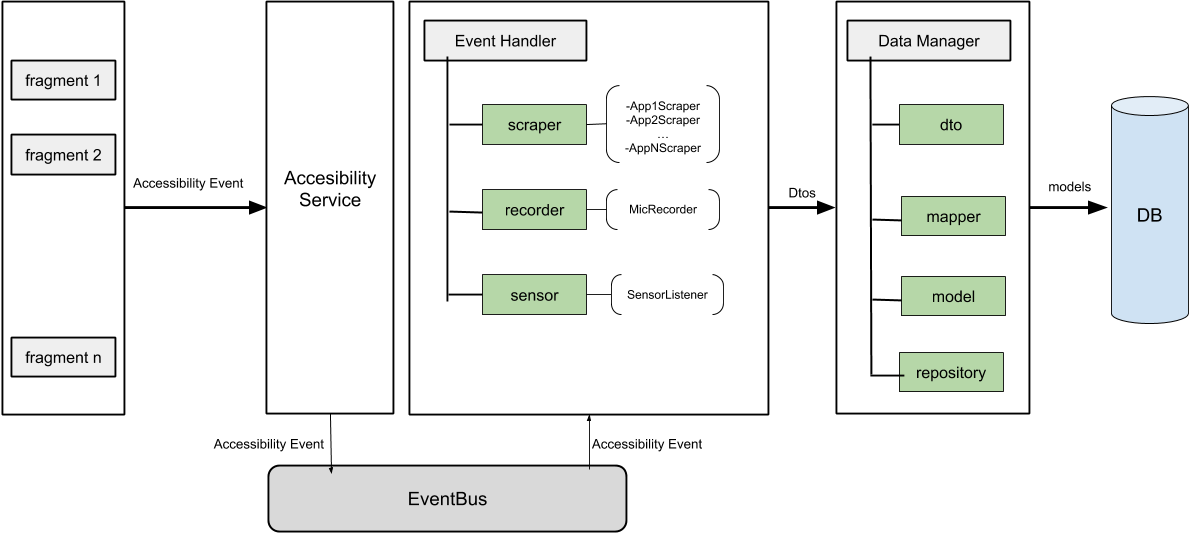
\includegraphics[width=1.3\textwidth,center]{pictures/architecture/arquitecturaGeneral03.png} 
%	\end{large}
	\caption[Arquitectura detallada]{Arquitectura detallada}
\end{figure}
%%% ------  
En primer lugar nos encontramos la ui que alimenta al servicio de accesibilidad con eventos. Este servicio se encarga de meterlos en un bus de forma que el manejador pueda recogerlos y computarlos. 
\newline \newline
Este tratamiento que realiza el manejador no es otro que, en función de la app que lo lanzó llamar a las clases implicadas en su tratamiento.
\newline \newline
Expliquemos más despacio en que consite esto. El manejador, como se ha dicho en alguna ocasión, analiza el package name del evento, este package name nos permite identificar el elemento del sistema android que lanzó el evento, ya sean relacionados con la aplicación en foco en ese momento como los relacionados con el uso de sensores del teléfono. 
\newline \newline
Los eventos de las aplicaciones serán tratados por los scrapers. Estos extraerán la información pertinente y la encapsularán en dtos. 
\newline \newline
Con los sensores la historia es diferente, puesto que la escucha de los mismos está ligada a la implementación de sendos listeners que recogen la información que van generando. En un apartado diferente entra la escucha del micrófono, puesto que para respetar la privacidad del usuario sólo se lanzará la captura de audio cuando un evento relacionado con la misma sea lanzado. Nos referimos a casos concretos del uso del móvil como comandos de voz, notas de audio, etc. 
\newline \newline
En la parte del Data Manager nos encontramos a las entidades y a los responsables de mover esas entidades a lo largo de la arquitectura. 
\newline \newline
Así nos encontramos con el paquete repository, encargado de la persistencia en base de datos de las entidades. Entidades como dtos (para la comunicación de información desde el manejador al data manager) y mappers, que realizarán la conversión de dtos a modelos, entidad aceptada por el repository para la persistencia en la base de datos. 
\newline \newline
De esta manera nos encontramos con 4 capas separadas por funcionalidad y con independencia lógica entre ellas, puesto que cada una está consagrada a una tarea particular (recibir eventos, computarlos, persistirlos). 
\newline \newline
La lógica de negocio del sistema se encuentra, sin duda, en la capa correspondiente al manejador, donde deberemos de echar un esfuerzo de implementación considerable para manejar todo el flujo de información. 
%%% ------


\chapter{Implementación y desarrollo}

%~\ref{fig:Calculo IDLE-PC} este valor es calculado automáticamente por el programa, algo que no pasa en versiones anteriores de este, donde se calculan varios valores que se muestran al usuario para que este seleccione uno de ellos.
%\begin{figure}[h]
%\centering
%\caption[Calculo IDLE-PC]{Calculo IDLE-PC}
%\label{fig:Calculo IDLE-PC}
%\end{figure}


\chapter{Conclusiones y trabajos futuros}


%%%%%%%%%%%%%%%%%%%%%%%%%%%%%%%%%%
%%%%%%%%%%% ANEXOS %%%%%%%%%%%%%%%
%%%%%%%%%%%%%%%%%%%%%%%%%%%%%%%%%%
%%\appendix
%%%\clearpage
%%\appendixpage
%%%\addappheadtotoc

%%%%%\chapter{Ejemplo de anexo}
%%%%%%Si no se desea incluir anexos, sólo hay que borrar este capítulo.
%%%%%\par



\pagebreak
%%%%%%%%%%%%%%%%%%%%%%%%%%%%%%%%%%
%%%%%%%%%% AL FINAL %%%%%%%%%%%%%%
%%%%%%%%%%%%%%%%%%%%%%%%%%%%%%%%%%
\thispagestyle{empty}
\pagestyle{empty}
%%%% https://en.wikibooks.org/wiki/LaTeX/Bibliography_Management
\addcontentsline{toc}{chapter}{Bibliografía}
\bibliographystyle{unsrt}
\bibliography{LocalBibliography.bib}
\end{document}
%%%%%\section{Secciones}
%%%%%Las secciones se crean con \textit{section}. Las subsecciones y %%%%subsubsecciones con \textit{subsection} y \textit{subsubsection}, %%%%respectivamente. Si se desea que alguna subsección en concreto no salga %%%%en el índice se pueden usar los mismos comandos añadiéndoles un %%asterisco al final (\textit{subsection*} y \textit{subsubsection*}).
%%\par

%%%%%\subsection{una subsección}

%%%%%%\subsection{otra subsección}
%%%%%%Excepteur sint obcaecat cupiditat non proident, sunt in culpa qui %%%%%%officia deserunt mollit anim id est laborum.
%%%%%%\subsubsection{subsubsecciones}
%%%%%%¡Por defecto las subsubsecciones no aparecen en el índice! Este %%%%%%comportamiento se puede cambiar.

%%%%%%\section{Citas y referencias}
%%%%%Para citar un texto hay que incluirlo en el fichero %%%%\textit{LocalBibliography.bib} de esta plantilla. Una vez hecho se %%%%%puede referenciar usando el comando \textit{cite}~\cite{LaTeX_tutorials}.
%%%%Para referenciar imágenes, secciones o tablas se usa el %%%%comando~\textit{ref}. Por ejemplo~\ref{fig:logoEpcc}. Es importante %%%%haber añadido una etiqueta con el nombre correspondiente al emenento a %referenciar.
%%%%%\par
%%%%%%Para facilitar la lectura, cuando se insertan citas y referencias %%%%%%es conveniente insertar un caracter de espacio sin salto de línea %%%%%%%%\textit{\~} antes del comando de cita o referencia.


%%%%%%\section{Imágenes}
%%%%%%Las imágenes se insertan así:

%%%%\begin{figure}[H]
%%%%%\centering
%%%%%
\includegraphics[width=0.6\textwidth]{pictures/logoEpcc.png}
%%%%%%\caption[Logo Epcc]{Logo Epcc.\\Fuente:http://www.unex.es/conoce-la-uex/centros/epcc/}
%%%%%%\label{fig:logoEpcc}
%%%%%%\end{figure}
